\documentclass[12pt]{article}
\usepackage[left=3.5cm,right=3.5cm,top=3.0cm,bottom=2.5cm]{geometry}
% \usepackage[some]{background}
\usepackage{fancyhdr}
\usepackage{listings}
\usepackage{xcolor}
\usepackage{tocloft}
\usepackage{pdflscape}
\usepackage{multicol}
\usepackage{amsmath}
\usepackage{setspace}
\usepackage{graphicx}
\usepackage{caption}
\usepackage{float}
\usepackage{units}
\usepackage{titlesec}
\usepackage{mathpazo}
%\usepackage[spanish]{babel}
\usepackage{url}
\usepackage{comment} 
% \usepackage{hyperref}
% \usepackage[hidelinks]{hyperref}
% \usepackage[spanish]{babel}
% \usepackage[utf8]{inputenc}

\usepackage{listings}

%\usepackage{footnotebackref}

\usepackage{natbib}

\usepackage{tikz}

% Define el color esmeralda 

\definecolor{emerald}{HTML}{00A99D}


\usepackage{setspace} % Always before hyperref -- Enable correct footnote link


\definecolor{gold}{HTML}{A69F69} % BCA954

\usepackage[font=scriptsize,labelfont=bf]{caption}

\usepackage{hyperref}
\hypersetup{
    colorlinks=true,
    linkcolor=emerald,
    filecolor=magenta,      
    urlcolor=cyan,
    pdfpagemode=FullScreen,
}
\urlstyle{same}

% ref packages
%\usepackage{nameref}
% folowing  must be in this order
%\usepackage{varioref}
%\usepackage{hyperref}
% \usepackage{cleveref}

% DEBUG
% \usepackage{showframe}
% {\selectfont}

%   SETTINGS
\onehalfspacing

\titleformat{\section}
{\normalfont\Huge\bfseries}{\thesection}{0em}{}
% \titleformat{\subsection}
% {\normalfont\large\bfseries}{\thesubsection}{1em}{}
% \titleformat{\subsubsection}
% {\normalfont\normalsize\bfseries}{\thesubsubsection}{1em}{}
% \titleformat{\paragraph}[runin]
% {\normalfont\normalsize\bfseries}{\theparagraph}{1em}{}
% \titleformat{\subparagraph}[runin]
% {\normalfont\normalsize\bfseries}{\thesubparagraph}{1em}{}



% Quitar los numeros de los headings de las secciones
\makeatletter
\renewcommand\thesection{}
\renewcommand\thesubsection{\@arabic\c@section.\@arabic\c@subsection}
\makeatother



\title{\vspace{-4ex}\Large{Implementación de la Componente Pricipal de la Plataform ENIGMA}}
\author{Luis Enrique Saborit Gonz\'alez}

\begin{document}

\pagenumbering{gobble}




% PORTADA ESPANOL

\tikz[remember picture,overlay] \node[opacity=1.0,inner sep=0pt] at (current page.center){
\includegraphics[width=\paperwidth,height=\paperheight]{imag/portada_clean.jpg}};

\vspace*{6.5cm}

\begin{center}
    \textcolor{gold}{\textbf{Departamento de Ciencia\\ de la Computaci\'on}}
\end{center}

\vspace*{0.5cm}

\begin{center}
    \Huge{\textbf{TRABAJO DE DIPLOMA}}
\end{center}


\vspace*{1cm}

\begin{center}
    \Large{\textbf{T\'itulo:} Implementación de algoritmos de aprendizaje para detección de eventos en plataformas basadas en tecnología IoT Semántica.}
\end{center}

\vspace*{1cm}

\begin{center}
    \large{\textbf{Autor:} Jos\'e Luis S\'anchez Ch\'avez }
\end{center}

\begin{center}
    \large{\textbf{Tutor:} Dr.C. Daniel Gálvez L\'io}
\end{center}

\begin{center}
    \large{\textbf{Tutor:} Dr.C. Amed Abel Leiva Mederos}
\end{center}

\vspace*{0.3cm}

\begin{center}
    \textbf{\textcolor{gold}{Santa Clara, noviembre 2022 \\ Copyright\textcopyright UCLV}}
\end{center}


\clearpage





% PORTADA INGLES

\newpage


\tikz[remember picture,overlay] \node[opacity=1.0,inner sep=0pt] at (current page.center){
\includegraphics[width=\paperwidth,height=\paperheight]{imag/portada_clean.jpg}};


\vspace*{6.5cm}

\begin{center}
    \textcolor{gold}{\textbf{Department of \\ Computer Science}}
\end{center}

\vspace*{0.5cm}

\begin{center}
    \Huge{\textbf{DIPLOMA THESIS}}
\end{center}


\vspace*{1cm}

\begin{center}
    \Large{\textbf{Title:} Implementation of learning algorithms for event detection in IoT Semantic technology-based platforms.}
\end{center}

\vspace*{1cm}

\begin{center}
    \large{\textbf{Autor:} Jos\'e Luis S\'anchez Ch\'avez }
\end{center}

\begin{center}
    \large{\textbf{Tutor:} Dr.C. Daniel Gálvez L\'io}
\end{center}

\begin{center}
    \large{\textbf{Tutor:} Dr.C. Amed Abel Leiva Mederos}
\end{center}

\vspace*{0.3cm}

\begin{center}
    \textbf{\textcolor{gold}{Santa Clara, november 2022 \\ Copyright\textcopyright UCLV}}
\end{center}


\clearpage


\newpage

\pagenumbering{roman}
\setcounter{page}{3}

\vspace*{10cm}
\noindent Este documento es Propiedad Patrimonial de la Universidad Central “Marta Abreu” de Las Villas, y se encuentra depositado en los fondos de la Bi\-blio\-te\-ca Universitaria “Chiqui Gómez Lubian” subordinada a la Dirección de In\-for\-ma\-ción Científico Técnica de la mencionada casa de altos estudios.

Se autoriza su utilización bajo la licencia siguiente: \newline
\textbf{Atribución - No Comercial - Compartir Igual}

\begin{figure}[H]
    
\includegraphics[width=5cm]{imag/license.png}
\end{figure}

Para cualquier información contacte con:

\noindent  Dirección de Información Científico Técnica. Universidad Central “Marta\\ Abreu” de Las Villas. Carretera a Camajuaní. Km 5\nicefrac{1}{2}. Santa Clara. Villa Clara. Cuba. CP. \texttt{54 830}

\noindent Teléfonos.: \texttt{+53 01 42281503-14190}

\newpage

\vspace*{4cm}

\begin{figure}[H]
    \centering
    
\includegraphics[width=3cm]{imag/logo.png}
\end{figure}

Hago constar que el presente trabajo fue realizado en la Universidad Central “Marta Abreu” de Las Villas como parte de la culminación de los estudios de la especialidad de Ciencia de la Computación, autorizando a que el mismo sea utilizado por la institución, para los fines que estime conveniente, tanto de forma parcial como total y que además no podrá ser presentado en eventos ni publicado sin la autorización de la Universidad.

\vspace{1cm}

\begin{center}
    \rule{4cm}{0.15mm}
    
    Firma del autor
\end{center}

Los abajo firmantes, certificamos que el presente trabajo ha sido realizado según acuerdos de la dirección de nuestro centro y el mismo cumple con los requisitos que debe tener un trabajo de esta envergadura referido a la temática señalada.

\vspace{1cm}

\begin{center}
    \rule{3cm}{0.15mm} \hspace{0.7cm} \rule{3cm}{0.15mm} \hspace{0.9cm} \rule{4.5cm}{0.15mm}
    
    Firma del tutor \hspace{0.8cm} Firma del tutor \hspace{1.2cm}  Firma del jefe del Dpto
\end{center}








\newpage
\vspace*{3cm}
\section*{Dedicatoria}
\vspace*{1cm}
\begin{flushright}
    \textit{ En este punto de mi carrera dedico mi tesis a mis padres, abuelos, hermanos y amigos que me apoyaron para culminar esta meta. }    
\end{flushright}









\newpage
\vspace*{3cm}
\section*{Agradecimientos}
\vspace*{1cm}
\begin{flushright}
    \textit{
        Agradezco a la UCLV por su exigencia en mi formación profesional, a mi familia, por creer en mí y alentarme a terminar la carrera.   
    }
    \textit{    
        A mis tutores, los Doctores Daniel Gálvez L\'io  y Amed Abel Leiva Mederos, por su ayuda en la planificación, información y organización en este Trabajo de Fin de Grado.
    }
    \textit{
        Finalmente agradezco a la vida por todos los logros que me ha permitido alcanzar y por todos los que vendran.   
    }
\end{flushright}



\newpage


\begin{flushright}
    \vspace*{7cm}
    \textit{``El obstáculo se convierte en el camino'' \\ Marco Aurelio}
\end{flushright}

\begin{flushright}
    \vspace*{7cm}
    \textit{``Whatever will be, will be!'' \\ Innuendo, Queen}
\end{flushright}

\newpage
\vspace*{3cm}
\section*{Resumen}
\vspace*{1cm}

Cuando termine los siguientes capitulos





\newpage
\vspace*{3cm}
\section*{Abstract}
\vspace*{1cm}

Cuando termine los siguientes capitulos




\setcounter{section}{-1}


\newpage
\tableofcontents









\newpage



\vspace*{3cm}
\section{Introducci\'on}


\pagenumbering{arabic}

\vspace*{1cm}

\textit{“La Web Semántica no es de por sí compleja. El lenguaje de la Web Semántica, en su corazón, es muy, muy simple. Se trata solo de las relaciones entre las cosas. Tim Berners-Lee.
" \citep{ref31}}

\vspace*{0.6cm}


La tecnología \textbf{IoT} (Internet de las cosas) \footnote{\href{{https://es.wikipedia.org/wiki/Internet_de_las_cosas}}{\url{https://es.wikipedia.org/wiki/Internet_de_las_cosas}}} está transformando rápidamente la forma en que interactuamos con el mundo. Con la proliferación de sensores y dispositivos conectados, se está produciendo una explosión de datos a una escala sin precedentes. Sin embargo, la capacidad de procesar y extraer valor de estos datos se está convirtiendo en una tarea difícil: los humanos no estamos diseñados para procesar cantidades masivas de información y encontrar patrones de comportamiento. La computadora primero encontró su uso en acelerar el funcionamiento de grandes cálculos numéricos eficientemente. Ahora es necesario que las computadoras resuelvan otra incompetencia humana, analizar grandes volúmenes de datos y tomar decisiones con ellos. Es aquí donde la \textbf{Web Semántica} y la \textbf{Inteligencia Artificial} (IA) pueden jugar un papel crucial.

La \textbf{Web Semántica} es una extensión de la Web actual que tiene como objetivo hacer que la información en Internet sea más fácilmente procesable por las máquinas. La idea detrás de la Web Semántica es crear una estructura de datos común y compartida que permita a las máquinas procesar y comprender la información de manera más eficiente. Se basa en la idea de que la información en la Web se puede representar mediante ontologías, que describen los conceptos y relaciones relevantes en un dominio específico del problema. Las ontologías se utilizan para estructurar y etiquetar los datos en la Web de manera que sean fácilmente procesables por las máquinas. Utiliza varios estándares y tecnologías para lograr su objetivo. Uno de los estándares clave es RDF (Resource Description Framework) \footnote{\href{{https://es.wikipedia.org/wiki/Resource_Description_Framework}}{\url{https://es.wikipedia.org/wiki/Resource_Description_Framework}}} , que proporciona un marco para describir y etiquetar recursos en la Web. También utiliza tecnologías como SPARQL (Protocolo y Lenguaje de Consulta de RDF) \footnote{\href{{https://es.wikipedia.org/wiki/SPARQL}}{\url{https://es.wikipedia.org/wiki/SPARQL}}} , que permite a las máquinas hacer consultas complejas en los datos RDF, y RDFa (RDF en Atributos), que permite incrustar metadatos RDF en documentos HTML.

La \textbf{Web Semántica} tiene una amplia variedad de aplicaciones prácticas. En este trabajo, la combinaremos con una plataforma IoT, una forma de interconectar dispositivos en un sistema integrado para permitir la creación de ontologías y vocabularios específicos del dominio, lo que permite una comprensión más profunda y precisa de los datos de sensores y su contexto. Esto permite que los datos de sensores sean más fácilmente compartidos y procesados por diferentes sistemas y aplicaciones que utilizan diferentes lenguajes de programación y plataformas. Esta aplicación da lugar a un nuevo concepto conocido como \textbf{Web Semántica de las Cosas} (\textbf{SWoT} por sus siglas en inglés).

En la \textbf{Web Semántica de las Cosas}, se aplican estas tecnologías semánticas para permitir que los dispositivos IoT se comuniquen y colaboren de manera más efectiva y eficiente. Esto implica la creación de interfaces semánticas que permitan a los usuarios interactuar con los dispositivos IoT de manera más natural y sencilla. La aplicación de tecnologías semánticas en IoT ofrece varias ventajas, como una mejor interoperabilidad y compatibilidad entre dispositivos IoT, lo que permite una mayor eficiencia y productividad. Además, la integración de datos de diferentes fuentes y formatos permite una mejor toma de decisiones y la generación de nuevos conocimientos y oportunidades.

En la actualidad existen importantes plataformas basadas en tecnología IoT Semántica. Entre estas se incluyen:

\begin{enumerate}
    \item {
        \href{https://internetofthings.ibmcloud.com/}{IBM Watson IoT Platform:} Esta plataforma de IBM utiliza tecnologías semánticas para analizar y comprender grandes volúmenes de datos generados por dispositivos IoT. Permite la integración de datos de diferentes fuentes y el desarrollo de aplicaciones inteligentes.
    }
    \item {
        \href{https://www.oracle.com/internet-of-things/}{Oracle IoT Cloud:} Es una plataforma de IoT de Oracle que utiliza tecnología semántica para gestionar y analizar datos de dispositivos conectados. Permite la creación de aplicaciones inteligentes en diversos sectores como transporte, agricultura y ciudades inteligentes.
    }
\end{enumerate}

Las plataformas basadas en tecnología \textbf{IoT Semántica} son herramientas fundamentales para el procesamiento de datos en investigaciones. Estas soluciones informáticas permiten la integración de diversas tecnologías y métodos de procesamiento de datos en tiempo real, lo que facilita la detección de eventos y patrones en los datos y ayuda a los investigadores a obtener resultados más precisos y útiles. En nuestro país, la existencia de estas plataformas es escasa.

De lo expuesto anteriormente, se plantea como problema científico a resolver la implementación y integración de algoritmos de aprendizaje para detección de eventos en la plataforma basada en \textbf{IoT Semántica ENIGMA} que hasta el momento no es capaz de predecir y analizar datos en streaming, lo que dificultará su servicio como sistema de información. Esta plataforma fue desarrollada por alumnos y profesores de nuestra Universidad.

\vspace*{1cm}
\noindent \textbf{Objetivo General}
\vspace*{1cm}
%\noindent Objetivo General

Implementación de algoritmos de aprendizaje para detección de eventos en la plataforma basada en IoT Semantica ENIGMA, encargada del procesamiento de flujos de datos, con una arquitectura extensible y escalable.

\vspace*{1cm}
\noindent \textbf{Objetivos Espec\'ificos}

\begin{enumerate}
    \item {Desarrollar una ontología basada en IoT stream data para la gestión de la plataforma.
    }
    \item {
        Seleccionar los algoritmos de machine learning para la gestión del aprendizaje en la plataforma ENIGMA en concordancia con los tipos de datos que maneja el sistema.
    }
    \item {
        Desarrollar los algoritmos de aprendizaje para tareas de clasificación, regresión y similitud.
    }
    \item {
        Definir consultas sobre SPARQL combinando los algoritmos de aprendizaje.
    }
    \item {
        Validar la capacidad predictiva de los algoritmos mediante un caso de estudio.
    }
\end{enumerate}

Explicacion del contenido de los capitulos de la thesis. Cuando termine los siguientes capitulos.



\newpage
\vspace*{3cm}
\section[Plataformas para el Procesamiento de Datos]{\texorpdfstring{Cap\'itulo 1: \\ Plataformas para el Procesamiento\\ de Datos}{Cap\'itulo 1: Plataformas para el Procesamiento\\ de Datos}}
\vspace*{1cm}

\begin{figure}[!ht]
    \centering
    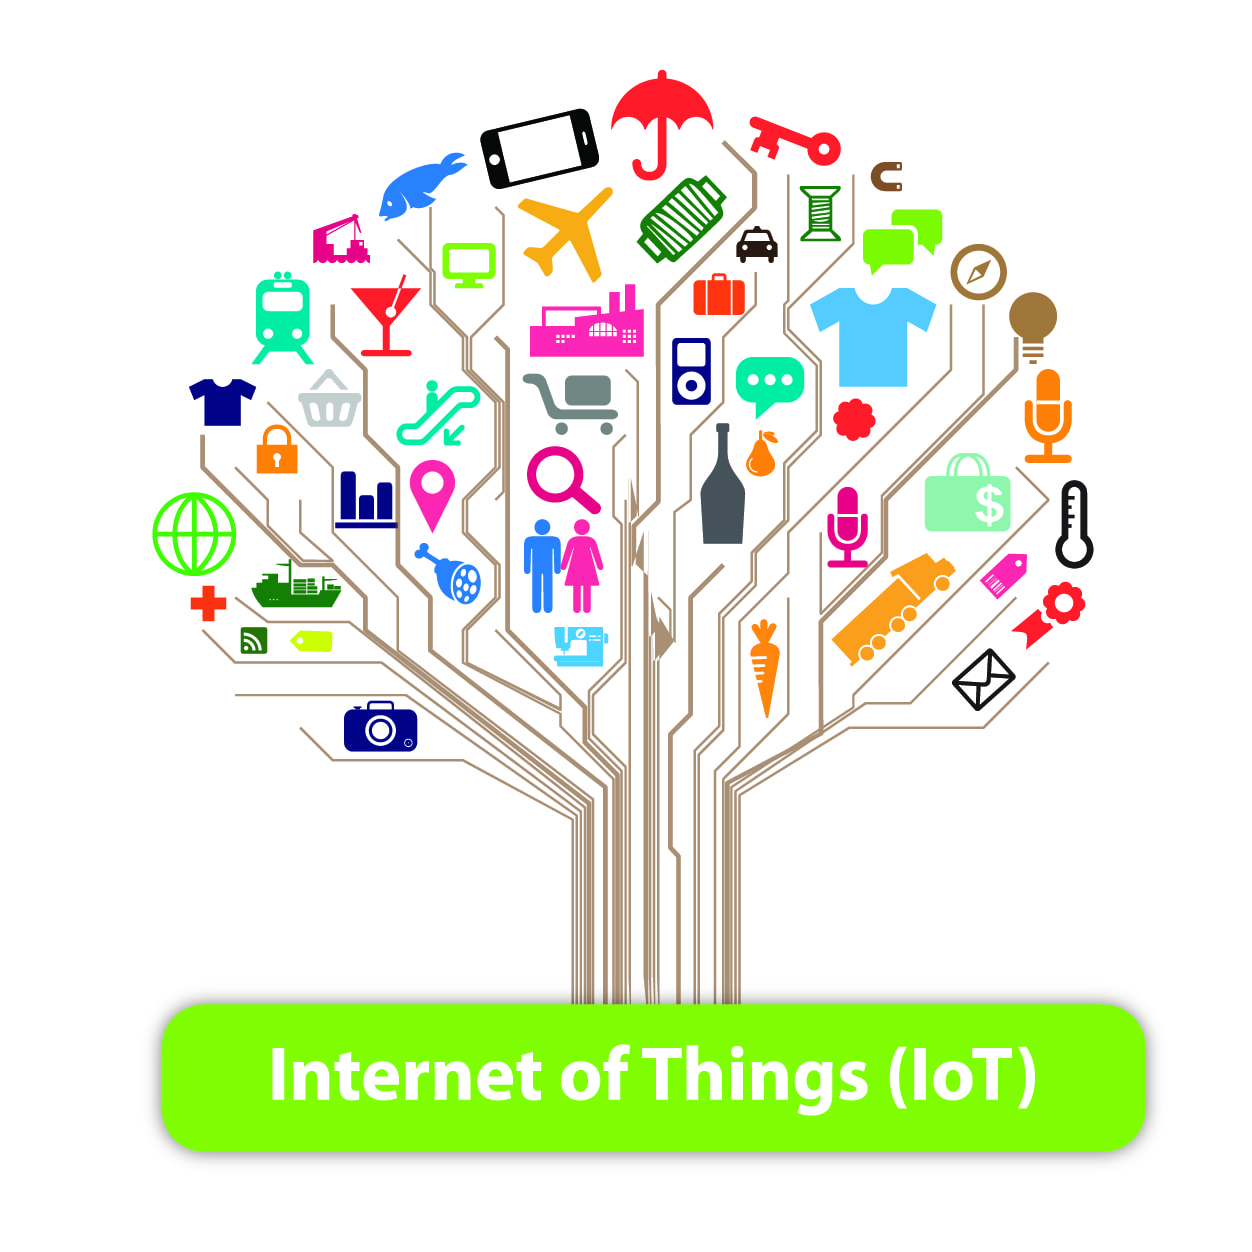
\includegraphics[width=0.95\textwidth]{imag/iot.jpg}
    \caption{Componentes del Internet de las Cosas \citep{ref39}}
    \label{fig:iot}
\end{figure}

Este capítulo aborda diversos temas relacionados con la detección de eventos en el contexto de la Internet de las cosas (IoT) y la integración de la \textbf{Web Semántica}, se presentan las tecnolog\'ias y los conceptos que conforman el marco teórico-referencial de este trabajo.

\subsection{Detección de Eventos}

Esta tecnología se basa en el análisis de datos y el uso de algoritmos y sistemas de inteligencia artificial para identificar patrones y anomalías que puedan indicar la presencia de un evento o situación específica.

La detección de eventos ofrece la capacidad de generar datos más oportunos en comparación con los datos disponibles a través de una red de sensores de infraestructura fija \citep{ref39}.

La detección de eventos es una tecnología que se utiliza para identificar y monitorear eventos o situaciones específicas en tiempo real. Estos eventos pueden ser desde situaciones de emergencia, como incendios o terremotos, hasta eventos relacionados con la salud, como brotes de enfermedades o epidemias.

Campos donde se aplica esta tecnología:

\begin{enumerate}
    \item {
        
        \textbf{Transporte: \citep{ref3} } la detección de eventos puede utilizarse para monitorear el tráfico y detectar situaciones de congestión, accidentes u otras incidencias que puedan afectar el flujo normal de vehículos.
    }
    \item {
       
        \textbf{Salud:} \citep{ref1} la detección de eventos puede utilizarse para identificar brotes de enfermedades o epidemias, analizando datos de hospitales, centros de salud y otras fuentes de información.
    }
    \item {
        \textbf{Seguridad:} \citep{ref4} se pueden utilizar cámaras de vigilancia y sistemas de análisis de video para detectar comportamientos sospechosos o actividades delictivas.
    }
\end{enumerate}




\subsubsection{Plataforma de detección de eventos en IoT Semántico.}

Las tecnologías semánticas pueden ayudar a gestionar, consultar y combinar sensores y datos de observación. Permitiendo así a los usuarios operar en niveles de abstracción por encima de los detalles técnicos de formato e integración, en lugar de trabajar con conceptos de dominio y restricciones de calidad. La semántica interpretable por máquina permite que agentes autónomos o semiautónomos ayuden a recopilar, procesar, razonar y actuar sobre los sensores y sus observaciones. Los datos de sensores vinculados pueden servir como un medio para interconectar datos de sensores con fuentes externas en la Web\citep{ref12}.

Una plataforma de detección de eventos en \textbf{IoT Semántico} es un sistema que utiliza tecnologías de Internet de las cosas (\textbf{IoT}) y semántica para identificar y analizar eventos en tiempo real.

Esta plataforma recopila datos de sensores y dispositivos conectados a la red \textbf{IoT}, y los procesa utilizando técnicas de análisis semántico para identificar patrones y eventos significativos. Estos eventos pueden ser cualquier tipo de cambio o suceso relevante, como la detección de un incendio, una fuga de agua, una caída de energía, entre otros.

La plataforma utiliza ontologías y modelos semánticos para describir los datos y los eventos, lo que permite una mejor comprensión y análisis de los mismos. Además, puede integrarse con otros sistemas o servicios para enviar notificaciones o tomar acciones en función de los eventos detectados.

Algunas características de una plataforma de detección de eventos en \textbf{IoT Semántico} pueden incluir:

\begin{enumerate}
    \item {
        
        Recopilación y procesamiento de datos en tiempo real.
    }
    \item {
       
        Análisis semántico de los datos para identificar patrones y eventos.
    }
    \item {
        Uso de ontologías y modelos semánticos para describir los datos y los eventos.
    }
    \item {
        Integración con otros sistemas o servicios para la notificación o toma de acciones.
    }
    \item {
        Capacidad para adaptarse y aprender de nuevos eventos o situaciones.
    }
    \item {
        Visualización y presentación de los eventos detectados en una interfaz gráfica intuitiva.
    }
        
\end{enumerate}

    
\subsection{La Web Sem\'antica} 
\label{ch}

\textit{La Web Semántica permitirá a las máquinas COMPRENDER documentos y datos semánticos, no el habla y los escritos humanos. \citep{ref10} } 

Una vez determinado que agregar sentido a los datos constituye una forma de resolver algunos de los desafíos que surgen al trabajar con flujos de datos y datos provenientes de sistemas IoT, se presentará formalmente el término Web Semántica para luego abordar el concepto de Ontología.

La Web Semántica es una extensión de la World Wide Web \footnote{\href{{https://es.wikipedia.org/wiki/World_Wide_Web}}{\url{https://es.wikipedia.org/wiki/World_Wide_Web}}} que busca agregar significado y contexto a la información disponible en Internet. Utiliza tecnologías y estándares como RDF (Resource Description Framework), OWL (Web Ontology Language) y SPARQL (Protocolo y Lenguaje de Consulta de RDF) para organizar y relacionar los datos de manera más estructurada. Los datos se representan mediante ontologías, que son modelos de conocimiento que describen conceptos, propiedades y relaciones entre ellos. Estas ontologías permiten a las máquinas entender y procesar la información de manera más inteligente, ya que pueden inferir nuevas relaciones y realizar consultas más complejas.

Berners-Lee describe la Web Semántica como \textit{“una extensión de la red actual en la que a la información se le da un significado bien definido, lo que permite a las computadoras y a las personas trabajar en cooperación"}\citep{ref10}. La información está estructurada de manera que las computadoras puedan establecer relaciones entre los recursos. Esas relaciones son lo que se conoce como datos vinculados.

La creación de metadatos estructurados de alta calidad y compartibles permite que su investigación sea más reconocible y vinculable a otros conjuntos de datos.

La idea central de la Web Semántica consiste en añadir metadatos semánticos y ontológicos. Estas informaciones adicionales se deben proporcionar de manera formal, para que así sea posible evaluarlas automáticamente por máquinas de procesamiento, lo cual conduce a experiencias de cliente más inteligentes y sin esfuerzo al brindar al contenido la capacidad de comprenderse y presentarse en las formas más útiles de acuerdo a las necesidades del mismo. El término fue acuñado por Timothy John Berners-Lee, el padre de la World Wide Web, quien logró incluir en esta última la información semántica necesaria. \citep{ref19}

Tiene aplicaciones en diversos campos, como la búsqueda de información más precisa y relevante, la integración de datos de diferentes fuentes, el descubrimiento de conocimiento oculto y la automatización de tareas repetitivas. Además, facilita la interoperabilidad entre sistemas y promueve la reutilización de datos.

\subsubsection{RDF}

RDF (Resource Description Framework) es una tecnología clave en el ámbito de la Web Semántica.

La segunda capa de la infraestructura de la Web Semántica es la Descripción del Recurso. RDF proporciona un modelo de datos simple para expresar declaraciones usando tripletas (sujeto, predicado, valor) y una sintaxis de serialización asociada en XML. El sujeto y el valor de la tripleta se pueden definir dentro del documento actual o consultar a otro recurso en la Web. El predicado puede ser cualquier XML (espacio de nombres, calificados). Para hacer declaraciones sobre una colección de recursos, RDF especifica un simple modelo de contenedor, secuencias de modelado (ordenadas), bolsas (desordenadas) y listas de alternativas. \citep{ref10}

El Marco de descripción de recursos (RDF) es una base para procesar metadatos; proporciona interoperabilidad entre aplicaciones que intercambian información comprensible para máquinas en la Web. RDF enfatiza las facilidades para permitir el procesamiento automatizado de recursos web. RDF se puede utilizar en una variedad de áreas de aplicación; por ejemplo: en el descubrimiento de recursos para proporcionar mejores capacidades de búsqueda, en la catalogación para describir el contenido y las relaciones de contenido disponibles en un sitio web, página o biblioteca digital, mediante agentes de software inteligentes para facilitar el intercambio y compartición de conocimientos, en la calificación del contenido, en la descripción de colecciones de páginas que representan una única lógica, para describir los derechos de propiedad intelectual de las páginas web y para expresar las preferencias de privacidad de un usuario, así como las políticas de privacidad de un sitio web. RDF con firmas digitales será clave para construir la "Web de confianza" para el comercio electrónico, la colaboración y otras aplicaciones.
\citep{ref46}

Un conjunto de declaraciones RDF utiliza un vocabulario particular que define las propiedades y tipos de datos que son significativos para la aplicación en cuestión. Como parte de su lenguaje de esquema, RDF-S también define algunos conceptos predefinidos, incluidas primitivas para modelar una clase/subclase jerarquía, relaciones entre clases ("propiedades") y restricciones de dominio/rango en tales propiedades. Tenga en cuenta que si bien el modelo RDF por sí solo proporciona simplemente un conjunto de triples, RDF-S ya es suficientemente expresivo para describir una jerarquía de clases que permite algunas consultas útiles y soporte de razonamiento. Por ejemplo, se podría consultar un sistema RDF-S en cuanto a si una instancia determinada pertenece a una clase específica, qué propiedades (heredadas). \citep{ref10}

Al utilizar RDF en la Web Semántica, se pueden lograr varios beneficios:
\citep{ref46}
\begin{enumerate}
    \item {
        
        \textbf{Interoperabilidad:} La RDF permite enlazar datos de diferentes fuentes y dominios, lo que facilita la integración de información y promueve la interoperabilidad entre aplicaciones y sistemas.
    }
    \item {
       
        \textbf{Búsqueda y descubrimiento mejorados:} Al representar la información en forma de tripletas y enlazar los recursos mediante URIs (Identificadores Uniformes de Recursos), se facilita la búsqueda y el descubrimiento de información relevante en la web.
    }
    \item {
        \textbf{Razonamiento y deducción:} Las ontologías y vocabularios basados en RDF permiten definir reglas y relaciones más complejas entre los datos, lo que facilita el razonamiento y la deducción automática sobre la información.
    }
    \item {
        \textbf{Integración de datos heterogéneos:} La RDF proporciona un marco flexible para integrar datos de diferentes formatos y fuentes, lo que facilita la combinación de información estructurada y no estructurada.
    }
    \item {
        \textbf{Compartir y reutilizar datos:} Al representar los datos en un formato estándar y basado en la web, se promueve el intercambio y la reutilización de información, lo que fomenta la colaboración y la construcción de aplicaciones más inteligentes.
    }
        
\end{enumerate}

\subsubsection{Sparql}

SPARQL (SPARQL Protocol and RDF Query Language) es el lenguaje estándar para consultar datos RDF. \citep{ref21}

SPARQL se utiliza para buscar, recuperar y manipular datos semánticos en forma de tripletas RDF. Permite realizar consultas flexibles y potentes que pueden recuperar información específica de un grafo RDF.

Cada vez más personas utilizan el lenguaje de consulta SPARQL (pronunciado "sparkle") para extraer datos de una colección cada vez mayor de datos públicos y privados. Ya sea que estos datos formen parte de un proyecto de web semántica o de una integración de dos bases de datos de inventario en diferentes plataformas detrás del mismo firewall, SPARQL está facilitando el acceso a ellos. En palabras del director del W3C e inventor de la web, Tim Berners-Lee, \textit{"Tratar de utilizar la Web Semántica sin SPARQL es como intentar utilizar una base de datos relacional sin SQL. SPARQL no fue diseñado para consultar datos relacionales, sino para consultar datos que se ajusten al modelo de datos RDF."} \citep{ref25}

Algunos conceptos clave en SPARQL son:

\begin{enumerate}
    \item {
        
        \textbf{Patrones de tripleta:} Las consultas \textbf{SPARQL} se construyen utilizando patrones de tripleta que consisten en una entidad (sujeto), una propiedad (predicado) y un valor (objeto). Estos patrones se utilizan para especificar los criterios de búsqueda y recuperar los datos deseados.
    }
    \item {
       
        \textbf{SELECT:} La cláusula \textbf{SELECT} se utiliza para especificar las variables que se desean recuperar en la consulta. Estas variables pueden ser sujetos, predicados u objetos en las tripletas.
    }
    \item {
        \textbf{WHERE:} La cláusula \textbf{WHERE} se utiliza para especificar los patrones de tripleta y las condiciones de búsqueda en la consulta. Aquí es donde se definen los criterios de búsqueda y se filtran los resultados.
    }
    \item {
        \textbf{FILTER:} La cláusula \textbf{FILTER} se utiliza para aplicar condiciones adicionales a los resultados de la consulta, como comparaciones, expresiones regulares, funciones matemáticas, etc
    }
    \item {
        \textbf{PREFIX:} La cláusula \textbf{PREFIX} se utiliza para definir prefijos que simplifican la escritura de URIs largas en las consultas SPARQL.
    }
        
\end{enumerate}

Un ejemplo sencillo de una consulta SPARQL sería:

\begin{lstlisting}
      PREFIX rdf:
          <http://www.w3.org/1999/02/22-rdf-syntax-ns#>
      PREFIX foaf:
          <http://xmlns.com/foaf/0.1/>

      SELECT ?name ?email
      WHERE {
          ?person rdf:type foaf:Person .
          ?person foaf:name ?name .
          ?person foaf:email ?email .
      }
\end{lstlisting}

En este ejemplo, buscamos personas en un grafo RDF que tienen un nombre y una dirección de correo electrónico. La consulta recupera las variables "?name" y "?email" de las tripletas que coinciden con los patrones especificados.

SPARQL proporciona una forma poderosa de consultar y recuperar datos semánticos en la Web Semántica, permitiendo la búsqueda y el análisis de información estructurada en RDF de forma eficiente.


\subsubsection{Starql}
STARQL (Lenguaje de consulta basado en razonamiento para streaming y acceso a ontologías temporales). STARQL está diseñado como un marco de consulta de flujo expresivo y flexible que ofrece la posibilidad de incorporar diferentes lógicas de descripción (temporales) como lenguajes de consulta de filtro sobre ontologías y, por lo tanto, puede usarse dentro del paradigma OBDA (Acceso a datos basado en ontologías en el sentido clásico) y dentro del paradigma ABDEO (Acceso a Big Data a través de Ontologías Expresivas). \citep{ref47}

STARQL es un lenguaje de consulta basado en razonamiento utilizado en el contexto de ontologías temporales y transmisiones (streams) en la Web Semántica.

STARQL combina las capacidades de consulta de SPARQL con la capacidad de razonamiento temporal y la capacidad de trabajar con flujos de datos continuos en tiempo real. Permite realizar consultas complejas que involucran datos temporales y flujos de datos continuos, y también permite el razonamiento basado en ontologías temporales.

Con STARQL, es posible realizar consultas que involucren la evolución temporal de los datos, como consultas que buscan información en un intervalo de tiempo específico, consultas que rastrean cambios en los datos a lo largo del tiempo, o consultas que combinan datos estáticos y flujos de datos en tiempo real.

Este lenguaje se basa en la especificación de ontologías temporales que definen conceptos y relaciones temporales, así como en la capacidad de razonamiento para inferir conocimiento basado en estas ontologías. STARQL permite la expresión de consultas que involucran tanto la estructura de la ontología como la dimensión temporal de los datos.

\subsubsection{Ontologia}

En la sección \ref{ch} se introdujo informalmente el concepto de ontología. En esta sección se abordará dicho concepto con mayor profundidad.

En filosofía, el concepto de ontología es una teoría sobre la naturaleza de la existencia, es decir, qué tipos de cosas existen. La ontología, como disciplina, estudia estas teorías. Los investigadores de Inteligencia Artificial y la Web han adoptado el término en su propio lenguaje técnico, y para ellos una ontología es un documento o archivo que define formalmente las relaciones entre los términos \citep{ref10}. 

Una ontología típica está compuesta por: \citep{ref10}
\begin{enumerate}
    \item {
    
        \textbf{Una taxonomía:} que define todas las clases de objetos y las relaciones que se establecen entre ellos.
    }
    \item {
       
        \textbf{Reglas de inferencia:} una ontología puede expresar la regla "si un código de ciudad está asociado con un código de estado y una dirección utiliza ese código de ciudad, entonces esa dirección tiene asociado el código de estado". Una aplicación que utiliza estos datos puede inferir que, si se proporciona un código de ciudad específico, esa dirección debe estar en una provincia o estado en particular. La computadora no "entiende" realmente ninguna parte de esta información, pero ahora puede manipular los términos de manera mucho más efectiva.
        }
        
\end{enumerate}

Un problema común es cuando se trabaja con dos bases de datos que usan diferentes identificadores para un mismo concepto, por ejemplo, cuando se trabaja con la información sobre dónde vive una persona. Dicha información puede ser representada tanto por un nombre como por un código postal, y se quiere comparar o modificar la información a través de las dos bases de datos, se tiene que saber que estos dos términos se utilizan para referirse a la misma cosa. Una solución a este problema la proporcionan las ontologías.

En resumen, la ontología en el campo de la computación es una herramienta para representar y organizar el conocimiento de manera formal y estructurada, permitiendo a las máquinas comprender y procesar la información de manera más eficiente.

\subsubsection{Ontologías para la IoT Semántica}

En el campo de la Internet de las cosas semántica (IoT Semántica), las ontologías juegan un papel fundamental para representar y organizar el conocimiento relacionado con los dispositivos, sensores, actuadores y datos generados en un entorno IoT.

Las ontologías en la IoT Semántica permiten establecer una estructura común y un lenguaje de representación compartido para describir los diferentes elementos y sus relaciones dentro de un sistema IoT. Esto facilita la interoperabilidad entre los dispositivos y aplicaciones, así como la integración de datos provenientes de diferentes fuentes.

Algunas ontologías comúnmente utilizadas en la IoT Semántica incluyen:

\begin{enumerate}
    \item {
       
       \textbf{SSN (Semantic Sensor Network Ontology):} Esta ontología se utiliza para describir y modelar los sensores, actuadores y observaciones en un entorno IoT. Proporciona una representación formal de las propiedades, capacidades y mediciones de los sensores, así como las relaciones entre ellos.\citep{ref49}
    }
    \item {
        \textbf{WoT (Web of Things Ontology):} Esta ontología se utiliza para describir y modelar los dispositivos conectados a través de la web en un entorno IoT. Proporciona una representación formal de las capacidades, servicios y características de los dispositivos, así como las relaciones entre ellos.\citep{ref48}
    }
    \item {
        \textbf{SSN-XG (Semantic Sensor Network Incubator Group):} Esta ontología se utiliza para extender la ontología SSN y proporcionar una representación más detallada de los sensores y observaciones en un entorno IoT. Incluye conceptos como calibración, precisión, incertidumbre y contexto.\citep{ref23}
    }
        
\end{enumerate}

Estas ontologías, junto con otras específicas del dominio, permiten una mejor comprensión y procesamiento de la información generada en un entorno IoT, lo que facilita la implementación de aplicaciones y servicios inteligentes basados en IoT.


\subsection{Data Strems}

Los streams de datos se refieren a un flujo continuo de datos que se transmite o se recibe. Puede estar en varias formas, como audio, video o texto, y generalmente se utiliza para la comunicación en tiempo real o la transferencia de datos. Los flujos de datos se encuentran comúnmente en aplicaciones como transmisiones en vivo, juegos en línea, videoconferencias y análisis de datos. Requieren una conexión de red estable y confiable para garantizar una transmisión ininterrumpida de datos.

\citep{ref50} definen un stream de datos como una secuencia infinita numerable de elementos. Existen diferentes modelos de flujos de datos que adoptan diferentes enfoques con respecto a la mutabilidad del flujo y la estructura de los elementos del flujo. El procesamiento de flujos se refiere al análisis de flujos de datos sobre la marcha para producir nuevos resultados a medida que se dispone de nuevos datos de entrada. El tiempo es un concepto central en el procesamiento de flujos: en casi todos los modelos de flujos, cada elemento de flujo está asociado con una o más marcas de tiempo de un dominio de tiempo determinado que podría indicar, por ejemplo, cuándo se generó el elemento, la validez de su contenido o cuándo estuvo disponible para su procesamiento.

\subsection{Algoritmos de Machíne Learning para IotStreman}

Hay varios algoritmos de Machine Learning que se pueden utilizar para el análisis de datos en tiempo real generados por dispositivos IoT (Internet of Things) en aplicaciones de streaming \citep{ref51}. Algunos de ellos incluyen:
\begin{enumerate}
    \item {
       
    \textbf{Regresión lineal:} Se utiliza para predecir valores continuos en función de variables de entrada. Puede ser útil para predecir tendencias o comportamientos en los datos de IoT.
        }
    \item {
    
    \textbf{Árboles de decisión:} Estos algoritmos dividen los datos en ramas de decisión basadas en características relevantes. Pueden ser utilizados para clasificar datos o tomar decisiones basadas en condiciones definidas.
        }
    \item {
        \textbf{Random Forest:} Es una combinación de múltiples árboles de decisión que generan predicciones y luego promedian los resultados. Puede ser útil para mejorar la precisión y reducir el sobreajuste.
        }
    \item{
        \textbf{K-means:} Es un algoritmo de agrupamiento que divide los datos en grupos basados en similitudes. Puede ser utilizado para segmentar los datos de IoT en diferentes grupos con características similares.
        }
    \item{
        \textbf{Redes neuronales:} Son modelos muy flexibles y potentes que pueden aprender patrones complejos en los datos. Pueden utilizarse para realizar predicciones o clasificaciones en tiempo real.
    }
        
\end{enumerate}

Estos son solo algunos ejemplos de los algoritmos de Machine Learning que se pueden utilizar en el análisis de datos de IoT en tiempo real. La selección del algoritmo adecuado dependerá de las características de los datos y los objetivos del análisis.

Actualmente se utilizan métodos de Machine Learning para analizar los datos de energía eléctrica facturada mensualmente en la Ciudad de Buenos Aires, durante el período 2010-2021 \citep{ref52}. Los objetivos son: determinar patrones en los datos utilizando el algoritmo K-Means y determinar las variables que más impactan en la energía facturada total a través del uso del algoritmo de Regresión Lineal. Como técnica de reducción de la dimensionalidad se utilizó el análisis de componentes principales. La investigación fue de tipo cuantitativa-explicativa, utilizando los datos de la Dirección General de Estadística y Censos de Buenos Aires, los cuales fueron analizados y preprocesados antes de la aplicación de los algoritmos; para generar los modelos se toma el 75\% de los datos para entrenamiento y el 25\% para la evaluación del modelo obtenido. Para el modelo de agrupamiento K-Means se determinó el K óptimo a través del método del codo, y se obtuvo que los datos de energía facturada total presentan una estacionalidad mensual. Para el modelo de Regresión Lineal se utilizaron las métricas R2, RMSE y MAE, y se obtuvo que las energías facturadas residencial, comercial e industrial, más el número de usuarios residenciales, son las variables que mayor impacto tienen sobre la energía eléctrica facturada total.

\subsection{Sistemas de Predicción de Eventos con IoT Semantic}

Los sistemas de predicción de eventos con IoT Semantic son aquellos que utilizan la tecnología de Internet de las cosas (IoT) y la semántica para predecir eventos futuros. Estos sistemas recopilan datos en tiempo real de sensores y dispositivos conectados, y los analizan utilizando algoritmos avanzados y modelos de aprendizaje automático.

La semántica se refiere a la capacidad de los sistemas de comprender el significado de los datos recopilados. Esto implica no solo analizar los valores numéricos o las mediciones, sino también comprender el contexto y las relaciones entre los diferentes datos. Por ejemplo, un sistema de predicción de eventos con IoT Semantic podría analizar datos de sensores de temperatura, humedad y presión atmosférica para predecir el clima futuro en una determinada ubicación.

Estos sistemas son especialmente útiles al predecir eventos futuros, ya que las organizaciones pueden tomar medidas preventivas o correctivas antes de que ocurran los eventos.

Algunos sistemas de predicción de eventos con IoT Semantic que se usan en la actualidad son:

\begin{enumerate}
    \item {
       
    \textbf{Sistema de detección y predicción de la calidad del aire y del agua para el monitoreo y control ambiental:} \citep{ref53} en explotación minera utilizando componentes IoT desarrollado por la Universidad Peruana de Ciencias Aplicadas (UPC).
    
    }
    \item {
    
    \textbf{Sistema para la recolección y reconocimiento de eventos domésticos mediante sensores de sonido en IoT:} \citep{ref54} permite reconocer eventos de sonido en un entorno doméstico. Para ello, en primer lugar, se realiza una recolección de muestras de sonido sobre diferentes eventos diarios que puedan ser recogidos por el dispositivo de sonido, tales como apertura de grifos de agua, puertas, electrodomésticos, etc. En segundo lugar, con un modelo basado en Deep Learning que permite clasificar los sonidos y es compatible con una ejecución en el dispositivo IoT, se obtiene una primera evaluación de su capacidad. En último lugar, se evalúa la posibilidad de integrar el modelo en tiempo real incluyendo un caso de estudio de una escena real. Desarrollado por la Universidad de Jaén (UJA).
    }
    \item {
        
    \textbf{Sistema para la aplicación de algoritmos de inteligencia artificial en sistemas de IoT orientado a la domótica:} \citep{ref55} La constante evolución de Internet ha propiciado una cuarta revolución industrial que lleva la transformación digital a industrias y empresas. Esto ha dado lugar a la aparición de tecnologías como la computación en la nube, las redes de Internet móviles, la robótica avanzada, el Internet de las cosas, los gemelos digitales y la inteligencia artificial, que han tenido un importante impacto socioeconómico. Con el paso del tiempo, estas tecnologías van llegando al día a día de las personas a través de los smartphones y diferentes dispositivos que se instalan en los hogares, como sensores de temperatura, sensores de calidad del aire, sensores de movimiento o sensores de incendio. Este trabajo pretende hacer uso de tecnologías en la nube para el procesamiento y almacenamiento de información, y para la ejecución de algoritmos de inteligencia artificial basados en datos obtenidos de dispositivos IoT. El propósito es crear un sistema capaz de ayudar al usuario final a tomar decisiones, mejorando su desempeño en su vida diaria. Desarrollado por la Universitat Oberta de Catalunya (UOC).



    }
        
\end{enumerate}

\subsection{Evaluacion de los Sistemas en el contexto de SemanticIOT}

La evaluación de los sistemas en el contexto de Semantic IoT (Internet de las Cosas Semántico) implica analizar el rendimiento y la efectividad de los sistemas que utilizan tecnologías semánticas en entornos de IoT.

Aquí hay algunos aspectos importantes a considerar:

\begin{enumerate}
    \item {
       
        \textbf{Interoperabilidad semántica:} \citep{ref8} Evaluar la capacidad del sistema para intercambiar y comprender datos semánticos entre diferentes dispositivos y plataformas dentro de un entorno IoT. Esto implica verificar si los dispositivos pueden comunicarse y entender los datos semánticos compartidos. Los proyectos de IoT plantean muchos desafíos, como la interoperabilidad entre aplicaciones de IoT debido a la gran cantidad de sensores, actuadores, servicios, protocolos y datos asociados con estos sistemas. La semántica resuelve este problema mediante el uso de anotaciones que definen el papel de cada elemento de IoT y reduce la ambigüedad de la información intercambiada entre los dispositivos.
    
    }
    \item {
    
        \textbf{Precisión semántica:} Evaluar la precisión con la que el sistema puede interpretar y representar los datos semánticos. Esto implica verificar si el sistema puede capturar de manera adecuada el significado y la semántica de los datos generados por los dispositivos IoT.
    }
    \item {
        
        \textbf{Eficiencia y escalabilidad:} Evaluar el rendimiento del sistema en términos de capacidad de procesamiento, almacenamiento y transmisión de datos semánticos en un entorno IoT. Esto implica verificar si el sistema puede manejar grandes volúmenes de datos semánticos y escalar eficientemente a medida que aumenta el número de dispositivos y la complejidad de las interacciones.

    }
    \item {
        
        \textbf{Seguridad y privacidad:} Evaluar las medidas de seguridad y privacidad implementadas en el sistema para proteger los datos semánticos generados por los dispositivos IoT. Esto implica verificar si el sistema cumple con los estándares y las mejores prácticas de seguridad, y si puede garantizar la confidencialidad, integridad y disponibilidad de los datos semánticos.
    }
    \item {
        
        \textbf{Usabilidad y experiencia del usuario:} \citep{ref10} Evaluar la facilidad de uso y la experiencia del usuario al interactuar con el sistema semántico IoT. Esto implica verificar si la interfaz de usuario es intuitiva, si se proporciona retroalimentación adecuada y si el sistema es accesible para diferentes usuarios.
    }
    \item {
        
        \textbf{Adopción y aceptación:} Evaluar la aceptación y adopción del sistema por parte de los usuarios y las organizaciones. Esto implica recopilar comentarios y opiniones de los usuarios para comprender su satisfacción con el sistema y su disposición a utilizarlo en entornos reales.
    }
        
\end{enumerate}




\newpage
\vspace*{3cm}
\section[Traffic: modelo para la deteccion de eventso de traficos]{\texorpdfstring{Cap\'itulo 2:\\ Traffic, modelo para la\\ deteccion de eventos de trafico}{Cap\'itulo 2:\\ Traffic, modelo para la\\ deteccion de eventos de trafico}}

\vspace*{1cm}

En este capitulo presentaremos un modelo semantico para la deteccion de eventos de Trafico como por ejemplo cuando hay un alto o un bajo nivel de trafico dentro de la ciudad

\subsection{ Datos captados por los sensores ubicados en Bruselas, \\ Belgica }

Para el sistema presentado se escogió la \textbf{API}\footnote{\href{{https://es.wikipedia.org/wiki/API}}{\url{https://es.wikipedia.org/wiki/API}}} \url{https://data.mobility.brussels/traffic/api/counts/}. Dicha decisión estuvo avalada por la buena documentación que presenta y el buen diseño de la misma, en cuanto a usabilidad y flexibilidad se refiere. Permite acceder a datos en tiempo real sobre el tráfico en Bruselas los sensores ofrecidos por dicho servicio están ubicados en carriles de distintas carreteras de la ciudad de Bruselas de Bélgica y para cada sensor se ofrecen sus observaciones en intervalos variables de 1, 5, 15 y 60 minutos.

Al utilizar esta API, puedes realizar diferentes tipos de consultas y obtener informacion especifica sobre el trafico en tiempo real. Algunos de los parametros que puedes utilizar en tus consultas incluyen:


\begin{itemize}
    \item {
       
        \textbf{"devices":} Con este parametro puedes obtener una lista con el nombre y la ubicación de los puntos de conteo de trafico.
    
    }
    \item {
    
        \textbf{"live":} Utilizando este parámetro, puedes obtener los datos más recientes de los detectores en vivo. Estos datos se actualizan constantemente.
    }
        
\end{itemize}

Además de los parámetros mencionados, también puedes especificar el formato de salida de los datos, como JSON o CSV. También existen otros parámetros opcionales, como "featureID" para solicitudes en vivo, que te permiten filtrar los datos según el nombre del sensor, y "interval" para especificar el intervalo de tiempo en minutos.

También se mencionan los servicios geoespaciales disponibles, como Web Map Service (WMS) y Web Feature Service (WFS), que te permiten acceder a datos geográficos relacionados con el tráfico.

Es importante tener en cuenta que la precisión de los datos puede variar. En condiciones de tráfico fluido, se espera un error inferior al 5\%, pero en situaciones de tráfico congestionado, este error puede aumentar hasta un 20-30\%. Además, se destaca que los dispositivos utilizados no están calibrados para medir la velocidad con precisión como los radares u otros dispositivos aprobados.

\subsection{Tráfico en Bruselas, Bélgica}

Bruselas es la capital de Bélgica y un importante centro político, económico y cultural. Como resultado, el tráfico en Bruselas puede ser bastante congestionado, especialmente durante las horas pico de la mañana y la tarde, cuando las personas se desplazan hacia y desde el trabajo. \citep{ref57}

La ciudad cuenta con una extensa red de carreteras y calles, pero debido a la densidad de población y la alta cantidad de vehículos, el tráfico puede volverse congestionado en ciertas áreas y en horas específicas. Algunas de las principales vías de transporte en Bruselas incluyen el Anillo de Bruselas (Ring), las autopistas E40 y E19, y las calles interiores que atraviesan la ciudad.

Además del tráfico de vehículos privados, Bruselas también tiene un sistema de transporte público bien desarrollado que incluye metro, tranvía y autobuses. Estos medios de transporte público pueden ser una opción conveniente para evitar la congestión del tráfico y moverse por la ciudad de manera eficiente.

Es importante tener en cuenta que las condiciones del tráfico pueden variar en función de varios factores, como eventos especiales, obras en la vía pública y condiciones climáticas.

\subsection{Pasos para crear la Ontologia para la prediccion de eventos de trafico}

El proceso de generación de ontologías para la predicción de eventos de tráfico implica varias etapas clave. A continuación, se presenta una descripción general de los pasos en este proceso:

\begin{itemize}
    \item {
       
        \textbf{Definición de requisitos:} En esta etapa se identifican y documentan los requisitos específicos del proyecto. Esto implica comprender las necesidades y objetivos del sistema o aplicación que se va a desarrollar, así como los requerimientos funcionales y no funcionales que deben ser cumplidos.
    }
    \item {
    
        \textbf{Selección de vocabularios para reutilización:} Se realiza una búsqueda y selección de vocabularios existentes que sean relevantes para el dominio del proyecto. Estos vocabularios pueden ser ontologías ya desarrolladas y disponibles públicamente.    }
    
    
    \item {
    
        \textbf{Implementación e integración de ontología:} Implementación e integración de ontología: En esta fase se procede a la implementación y desarrollo de la ontología. Esto implica definir las clases, propiedades y relaciones que representarán los conceptos del dominio y sus interacciones.   }

    
    \item {
    
        \textbf{Documentación:} Es importante documentar la ontología de manera clara y completa.   }
    

\end{itemize}

\subsubsection{Definición de requisitos}

Para la detección de eventos de tráfico, es necesario emplear ontologías especializadas que permitan su clasificación. Esto favorecera a la utilizacion de clases como IotStream y sus ontologias vinculadas, la clase IoTStream Analytics se puede utilizar en relación con el análisis de tráfico. Conocer la ubicación desplegada de los sensores también es vital para el análisis geoespacial, por lo que con la vinculación de IoT-Stream a geo:Point, esto se puede capturar utilizando coordenadas absolutas o ubicación relativa (utilizando iot-lite:relativeLocation).

Usaremos Neo4j para modelar y representar los datos en forma de grafo. Con Cypher lenguaje que nos ofrece esta base de datos realizaremos las consultas para buscar patrones especificos en el grafo, como identificar eventos de trafico relacionados con una ubicación geografica particular.

Al igual que en OEMA cada elemento de la ontologia debe nombrarse usando solo un termino para evitar la heterogenidad semantica. El idioma usado sera OWL-2 y los elementos de la ontología usaran como anotación las posturas de Camel Case (CamelCase).

\subsubsection{Selección de vocabularios para reutilización}

\subsubsection{Implementación e integración de ontologia}

\subsubsection{Documentación}


\begin{comment}

En este cap\'itulo se describen en profundidad las principales caracter\'isticas de la plataforma ENIGMA, teniendo como base de esta caracterizaci\'on el modelo \textbf{C4}. Tambi\'en se enumeran las principales clases que componen la implementaci\'on del sistema.    

\subsection{Caracter\'isticas Generales de la Plataforma}

Con la plataforma ENIGMA\footnote{\href{https://github.com/Saborit10/thesis}{https://github.com/Saborit10/thesis}} se busca implementar una soluci\'on enfocada en el procesamiento de flujos de datos, independientemente de la diversidad de tipos de mediciones y de la fuente de donde provienen estos, que sea flexible y de fácil puesta en marcha en un nuevo caso de uso. La plataforma es capaz de adaptarse a nuevos entornos, sin que sea necesario modificar el código fuente y, por ende, sin tener que compilarlo cada vez que se desee adaptar.

Adem\'as se desea que la plataforma maneje varias instancias o casos de uso simultáneamente, algo que no era posible en el sistema Traffic. Esto es un cambio de paradigma con respecto a su antecesora, ya que en este caso no se desea desplegar el sistema cada vez que se vaya a usar en un nuevo entorno, sino que se pretende usar la plataforma en varios entornos al mismo tiempo.

Para lograr esto, adem\'as de los conceptos \textbf{Sensor}, \textbf{Stream} y \textbf{Observation}, heredados del sistema Traffic, se introduce el concepto \textbf{Topic}, o asunto. Un asunto representa una instancia del sistema adaptado a un entorno espec\'ifico, con sus caracter\'isticas propias, las cuales son definidas cuando este se crea.  

ENIGMA se encarga de todo el procesamiento que es com\'un a las operaciones relacionadas con sensores y flujos de datos, dejando solo las tareas espec\'ificas al usuario que desea adaptar la plataforma a su caso de uso particular. 

El sistema est\'a construido en forma de servicios que se comunican entre s\'i mediante el paso de mensajes.  Este tipo de arquitectura nos permite desplegar la plataforma como un sistema distribuido. Adem\'as facilita el mantenimiento, las pruebas y los cambios de tecnolog\'ia en un servicio espec\'ifico.



\subsection{Descripci\'on del Entorno de la Plataforma}

En el dise\~no de la plataforma ENIGMA, se ha prestado especial atenci\'on a la simplificaci\'on de los pasos para la adaptaci\'on a un nuevo caso de uso.

\begin{figure}[!ht]
    \centering
    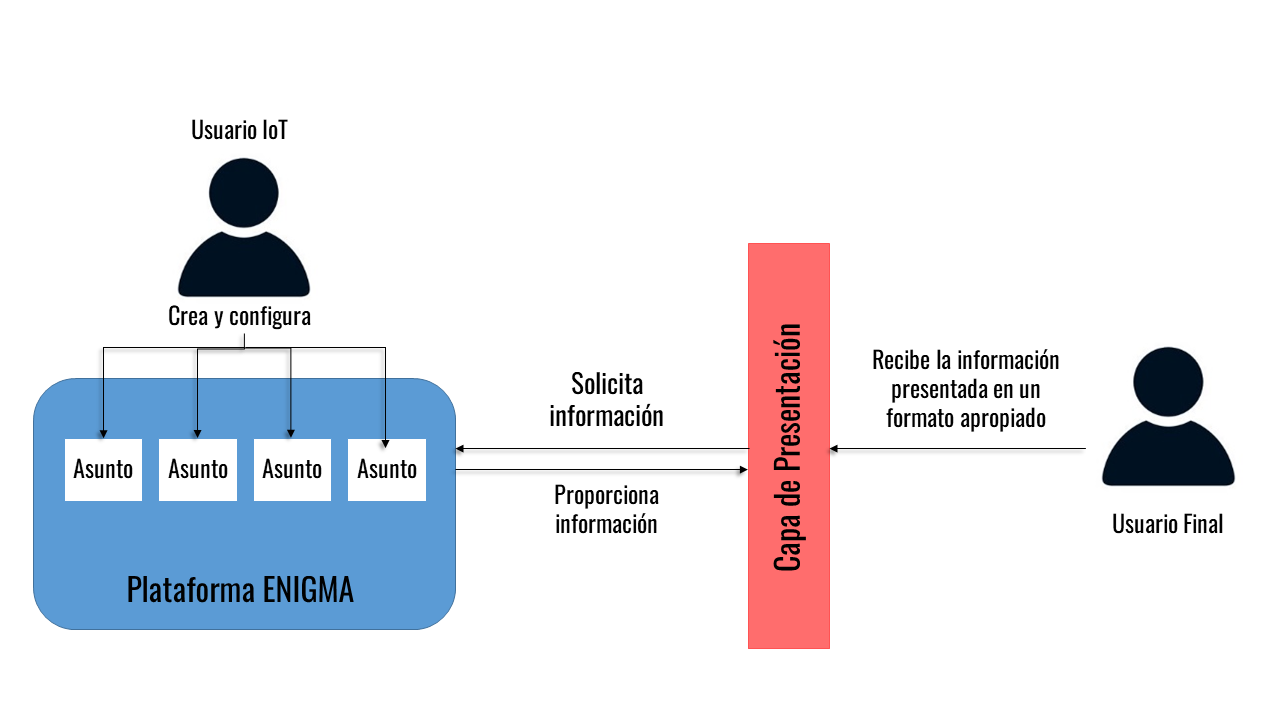
\includegraphics[width=\textwidth]{imag/esquema4.png}
    \caption{Diagrama de Contexto de la plataforma ENIGMA}
    \label{fig:diagrama_contexto}
\end{figure}

Como podemos ver en el diagrama de contexto (nivel $1$ del modelo \textbf{C4}) en la figura \ref{fig:diagrama_contexto}, existen dos tipos de usuario de la Plataforma ENIGMA. El primer tipo de usuario es el Usuario IoT, encargado de adaptar la plataforma a un caso de uso espec\'ifico. Para ello crea, configura y gestiona un asunto. Adem\'as puede crear componentes consumidores y servicios de anal\'iticas, sean estos internos o externos.

El segundo tipo de usuario es el usuario final. Este tiene un contacto indirecto con la plataforma y generalmente solo recibe la informaci\'on ya procesada y en un formato que facilite su comprensi\'on. La capa de presentaci\'on puede estar compuesta por uno o m\'as elementos consumidores: por ejemplo una p\'agina web, una aplicaci\'on de escritorio o un sistema de notificaciones.  





\subsection{Dise\~no de los Componentes de la Plataforma}

La plataforma consta de varios componentes, como se muestra en la figura \ref{fig:esquema_general}. Cada componente es independiente y varios de ellos se usan bajo demanda, o sea, solo si se necesita para el caso de uso concreto. A continuaci\'on se describen algunos de ellos, combinando los niveles $3$ y $4$ del modelo \textbf{C4}.

\begin{figure}[!ht]
    \centering
    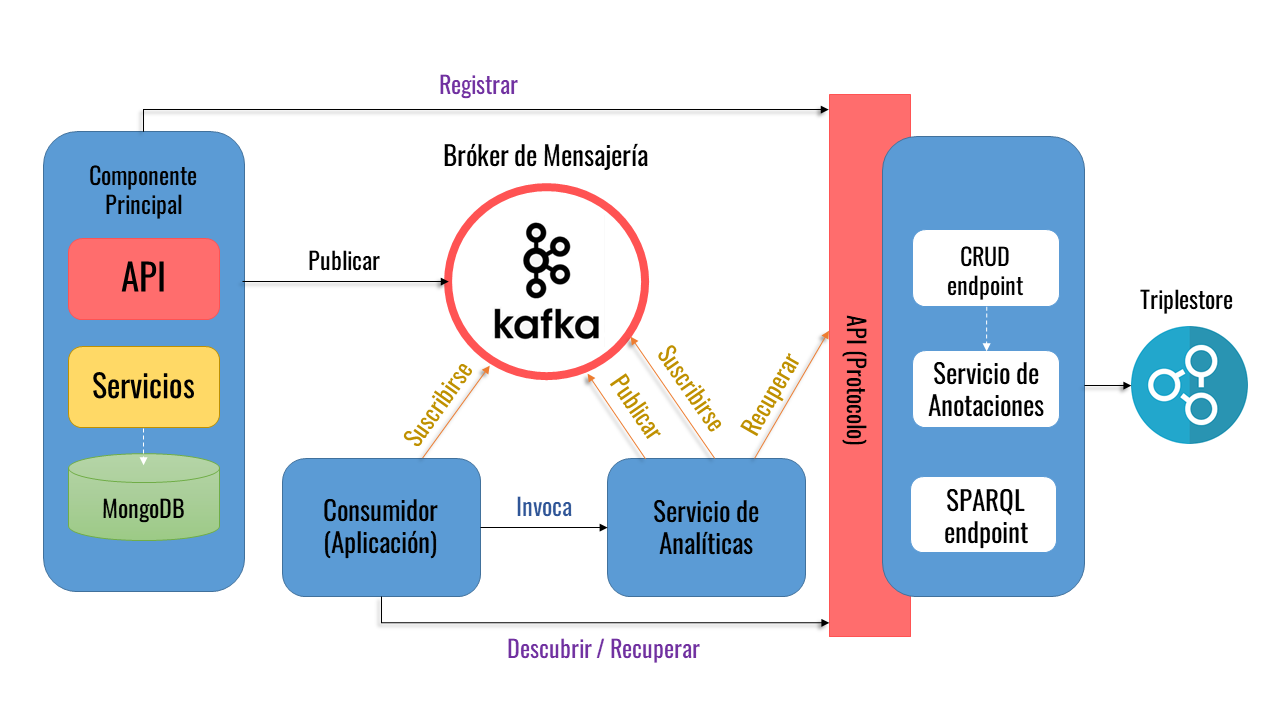
\includegraphics[width=\textwidth]{imag/esquema3.png}
    \caption{Esquema de los componentes de la plataforma ENIGMA}
    \label{fig:esquema_general}
\end{figure}

\subsubsection{Componente Principal}
El componente \textbf{Principal} está escrito en lenguaje Java y se usa el kit de herramientas \textbf{Vert.x} para lograr que las operaciones que realiza este componente se hagan de forma as\'incrona. Además, este kit se usa en el desarrollo de la API mediante la cual se introducen en el sistema los sensores, las \textit{streams} y las observaciones.

Este componente está compuesto por varios servicios. Estos son:

\begin{itemize}
    \item{
        \textbf{ApiService:} este servicio expone una \textbf{API HTTP} a la cual, usando el verbo POST se pueden publicar nuevos sensores, nuevos streams y observaciones. Estos datos deben ser publicados en un formato JSON específico para que puedan ser procesados por el sistema. La plataforma no se conecta directamente a la fuente de datos, sino que estos deben ser publicados a la API. De esta forma logramos abstraernos del formato original de los datos y podemos procesarlos sin  importar cual sea su fuente.

        La API tambi\'en expone m\'etodos que permiten obtener informaci\'on sobre los sensores y flujos de datos.
    }
    \item{
        \textbf{SensorService:} es un servicio que se ocupa de gestionar los sensores con los que trabaja cada \textbf{Topic} del sistema. Para ello utiliza una base de datos no relacional, m\'as especificamente un repositorio \textbf{MongoDB}. Los sensores se guardan en esta base de datos en formato JSON.
    }
    \item{
        \textbf{StreamService:} se encarga de gestionar los \textit{streams} que generan los sensores. Al igual que el \textbf{SensorService}, utiliza un repositorio \textbf{MongoDB} para guardar los datos en formato JSON. Además, este servicio puede realizar la b\'usqueda de un \textit{stream} determinado, dado el identificador del sensor donde se origina y la característica o \textit{feature} que le corresponde. Mediante este servicio también podemos borrar \textit{streams} del repositorio.
    }
    \item{
        \textbf{ObservationService:} este servicio se encarga de gestionar las observaciones y publicarlas al br\'oker de mensajer\'ia. Este es el procesamiento por defecto que se lleva a cabo con las observaciones. 
    }
    \item{
        \textbf{ObservationLoggingService:} es un servicio que registra todas las observaciones que son procesadas por el sistema en un repositorio \textbf{MongoDB}, para su posterior análisis. Por ejemplo, estos datos pueden ser usados para entrenar los algoritmos de Inteligencia Artificial que brinda \textbf{Stardog}, y se pueden usar en la plataforma.
        
        Normalmente estos datos no se guardan sino que son publicados con el componente \textbf{Br\'oker de Mensajer\'ia}.
    }
    \item{
        \textbf{TopicService:} es el servicio que se encarga de crear, modificar, buscar y eliminar los asuntos. Para ello los guarda en un repositorio \textbf{MongoDB} y en un objeto de tipo \textbf{TopicCollection} que es usado por todo el sistema. 
    }
\end{itemize}

\subsubsection{El Br\'oker de Mensajer\'ia}
El br\'oker de mesajer\'ia es el componente que se encarga de la comunicaci\'on entre los componentes del sistema, utilizando el patr\'on \textit{publish-subscribe}. Brinda facilidades para la detecci\'on y publicaci\'on de eventos en tiempo real.

Una de las modificaciones que se propone es sustituir el br\'oker basado en \textbf{Redis}, una base de datos en memoria, por uno basado en \textbf{Apache Kafka}, que es un sistema de transmisi\'on de mensajes. Entre las principales ventajas de \textbf{Kafka} \citep{ref32} tenemos:

\begin{itemize}
    \item {
        Mientras en \textbf{Redis} los datos son guardados en la forma \textit{clave-valor}, en \textbf{Kafka} son organizados en grupos llamados \textit{topics}, o temas. 
    }
    \item {
        Soporta paralelismo mediante la partición de los datos en el registro, donde múltiples consumidores pueden procesarlos al mismo tiempo, algo de lo que carece \textbf{Redis}.
    }
    \item {
        Mientras los mensajes publicados en \textbf{Redis} se entregan automáticamente a los suscriptores, en Kafka los mensajes publicados nunca se distribuyen directamente a los consumidores. Los consumidores deben suscribirse a los \textit{topics} y pedir los mensajes cuando est\'en listos para procesarlos. Adem\'as los mensajes en \textbf{Kafka} son retenidos un tiempo mucho m\'as largo que en \textbf{Redis}.
    }
    \item {
        \textbf{Kafka} está pensado para manejar grandes cantidades de datos. Permite utilizar tantos servidores como sea necesario y mantener hasta terabytes de datos durante un período de retención más largo que \textbf{Redis}, gracias a que almacena los datos en disco.
    }
\end{itemize}

La principal desventaja de \textbf{Apache Kafka} es su lentitud en comparación con \textbf{Redis}, debido a que guarda los mensajes incluso después de entregarlos.

En conclusi\'on, se propone usar \textbf{Kafka} en busca de fiabilidad, alto rendimiento, tolerancia a fallos y para manejar un volumen de datos enorme.


\subsubsection{Componente Consumidor}

El componente Consumidor se encarga de mostrar al usuario final los datos que han sido procesados. Este puede estar implementado, por ejemplo, como un cliente web para monitorear los eventos. 

Al igual que en el sistema Traffic, este componente es opcional y pueden existir varias implementaciones e instancias del mismo. Este elemento debe ser generalmente externo, aunque se puede desarrollar uno en la plataforma para mostrar los resultados de forma gen\'erica. 

Si se quiere ofrecer los datos sobre los eventos detectados a otros sistemas, entonces podemos consumir estos directamente desde el componente Br\'oker de Mensajer\'ia, o gestionar su consumo a través de una API.


\subsubsection{Servicio de Anal\'iticas}
Este componente detecta eventos en los flujos de datos y los publica al componente Br\'oker de Mensajer\'ia.

Los servicios de analíticas internos (o sea que pertenecen a la plataforma) se despliegan bajo demanda. Cualquier consumidor puede solicitar iniciarlos haciendo la petición correspondiente. Estos servicios pueden ser entrenados usando, por ejemplo, algoritmos de agrupamiento que sean desarrollados para la plataforma.

Debe hacerce primero una petici\'on para que el sistema comience a reunir datos durante un per\'iodo de tiempo, y as\'i entrenar los modelos de inteligencia artificial que est\'en disponibles.

Un servicio de anal\'iticas tambi\'en puede ser externo, y por ende, desarrollado por el usuario que desea adaptar la plataforma. En este caso se pueden obtener y publicar los datos a traves de las APIs, o mediante el br\'oker de mensajer\'ia. 

Para conectarse al br\'oker, primero debe hacerse una petici\'on a la API para pedir conectarse al sistema. Si la petición se responde de forma exitosa, entonces se recibir\'a como respuesta el nombre del canal del bróker de mensajería en el cual el servicio podr\'a comenzar a publicar los eventos detectados.

Los resultados que aporten estos servicios, o sea, los eventos detectados al ser publicados a la plataforma, constituyen a su vez nuevos \textit{streams} de datos a ser procesados. 

\subsubsection{Registro IoT}

El componente Registro IoT se encarga de almacenar la información referente a las entidades del sistema para luego enriquecer los datos. Como pasaba en el sistema Traffic, en este componente se delega todo el peso semántico del sistema, y puede ser consultado mediante la API que ofrece, o mediante el lengueje de consulta \textbf{SPARQL}.

A este componente pueden conectarse los componentes consumidores y los servicios de anal\'iticas (sean internos o externos a la plataforma), y adem\'as el componente principal, que se encarga de registrar datos acerca de sensores y \textit{streams}.

Los metadatos se almacenan en un \textit{triplestore} de tipo \textbf{Stardog}. Se decidió mantener esta implementación por su simpleza y útil panel de adminstración visual al cual se puede acceder desde una instancia ya sea local o remota \citep{ref3}.

La implementaci\'on de este componente debe ser muy parecida a la del sistema Traffic, solo hay que tener en cuenta abstraerse de los deferentes tipos de datos que se pueden procesar. 

El Registro IoT (figura \ref{fig:esquema_general}) contiene el \textit{endpoint} CRUD, que forma parte de la API que expone. Tambi\'en tiene como subcomponente al servicio de anotaciones, el cual se encarga de transformar los datos recibidos sobre los sensores y los \textit{streams} en documentos \textbf{RDF} para luego ser suministrados al \textbf{triplestore}, así como de proporcionar los \textbf{IRIs} correspondientes a las definiciones de dominio. El triplestore ofrecido por \textit{Stardog} implementa \textit{out of the box} el protocolo \textbf{SPARQL 1.1}, el cual representa el tercer sucomponente: el SPARQL \textit{endpoint} \citep{ref3}.


Se propone la creaci\'on de una API similar a la que implementa el sistema Traffic en su componente \textbf{IoT Registry}. Esta API debe ser lo suficientemente general para lograr la flexibilidad en cuanto a los tipos de datos que se pueden procesar y la cantidad de componentes internas y externas a la plataforma, e instancias de distinta naturaleza con las que se trabaja. Por ejemplo, debe posibilitar una comunicaci\'on fluida con los componentes de Servicios de Anal\'iticas externos a la plataforma.




\subsection{Principales Conceptos}

Los principales conceptos del dise\~no son \textbf{Sensor}, \textbf{Stream}, \textbf{Observation} y \textbf{Topic}. Estos son los elementos que definen caracter\'isticas espec\'ificas de las instancias o que representan la informaci\'on.

Un \textbf{Topic}, o asunto, representa una instancia del sistema, adaptada a un caso de uso. El concepto \textbf{Sensor} representa un sensor, o sea un dispositivo que genera un \textit{stream} en nuestra fuente de datos. Por su parte, un objeto \textbf{Stream} representa un \textit{stream} de datos generados por un sensor. Por \'ultimo, una observación es un resultado que produce un sensor en un instante de tiempo determinado. Un \textit{stream} est\'a compuesto por observaciones en orden cronol\'ogico. 

El valor de una observaci\'on puede ser de diferentes tipos dependiendo del caso de uso en el que se est\'e trabajando. Por ejemplo, puede tomar un valor entero, un valor decimal, o puede tomar uno de los valores de una lista de opciones conocidas. Tambi\'en se pueden modelar y programar nuevas clases que representen otros tipos de medici\'on sin tener que cambiar el c\'odigo, solo agregando nuevo. Esto garantiza la flexibilidad y extensibilidad de la plataforma.




\subsection{Implementaci\'on del Componente Principal}
% TODO

Cada uno de los pricipales conceptos de la plataforma se modela como una clase y se gestiona mediante un servicio. Adem\'as, sus datos se guardan en repositorios o son publicados al br\'oker.

A continuaci\'on se describen las principales clases y relaciones entre clases, que podemos encontrar en el sistema. Este es el nivel $4$ del modelo \textbf{C4}.

De cada \textbf{Topic} se guarda un identificador, un nombre, el autor, una descripción, el nombre de la base de datos donde vamos a guardar su informaci\'on correspondiente, un objeto \textit{factory} que sirve para crear instancias de la clase que representa el valor del resultado de una observaci\'on, y la frecuencia a la que se publican observaciones al sistema, medida en segundos.

\begin{figure}[!ht]
    \centering
    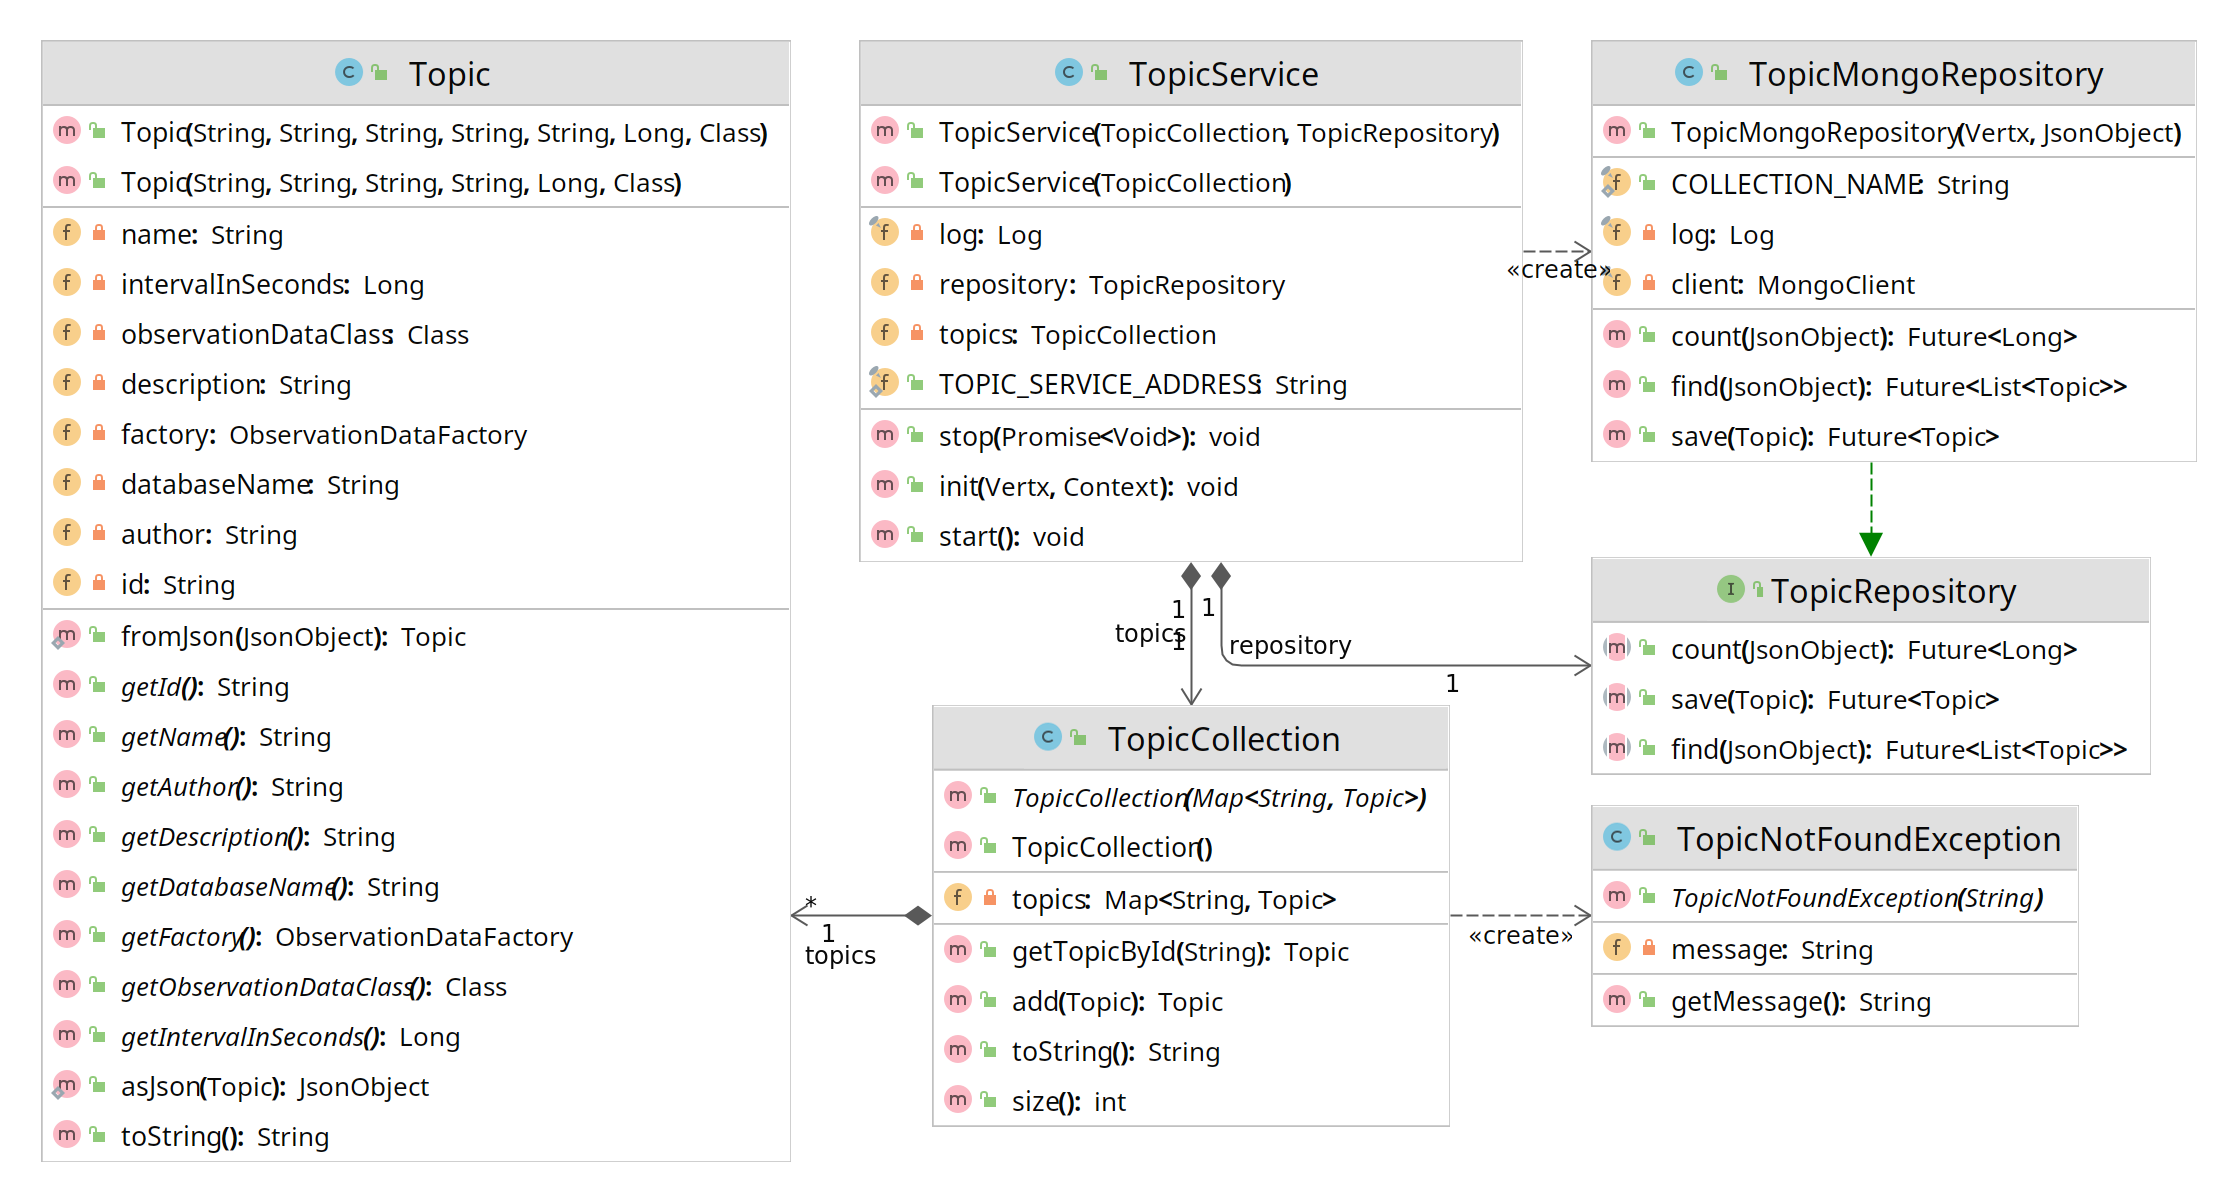
\includegraphics[width=\textwidth]{imag/uml_topics.png}
    \caption{Diagrama de clases relacionadas con los asuntos}
    \label{fig:uml_topic}
\end{figure}

Como podemos ver en la figura \ref{fig:uml_topic}, la clase \textbf{TopicService}, que representa el servicio que gestiona los asuntos en el sistema, posee un atributo de tipo \textbf{TopicCollection}, el cual es un conjunto de asuntos del sistema que se guarda en memoria. La interfaz \textbf{TopicRepository} define el comportamiento de un repositorio que guarda asuntos. Este comportamiento es implementado por la clase \textbf{TopicMongoRepository}. Para guardar un asunto en el repositorio, se serializa en formato JSON, tal como se muestra en la figura \ref{fig:topic}.

\begin{figure}[!ht]
    \centering
    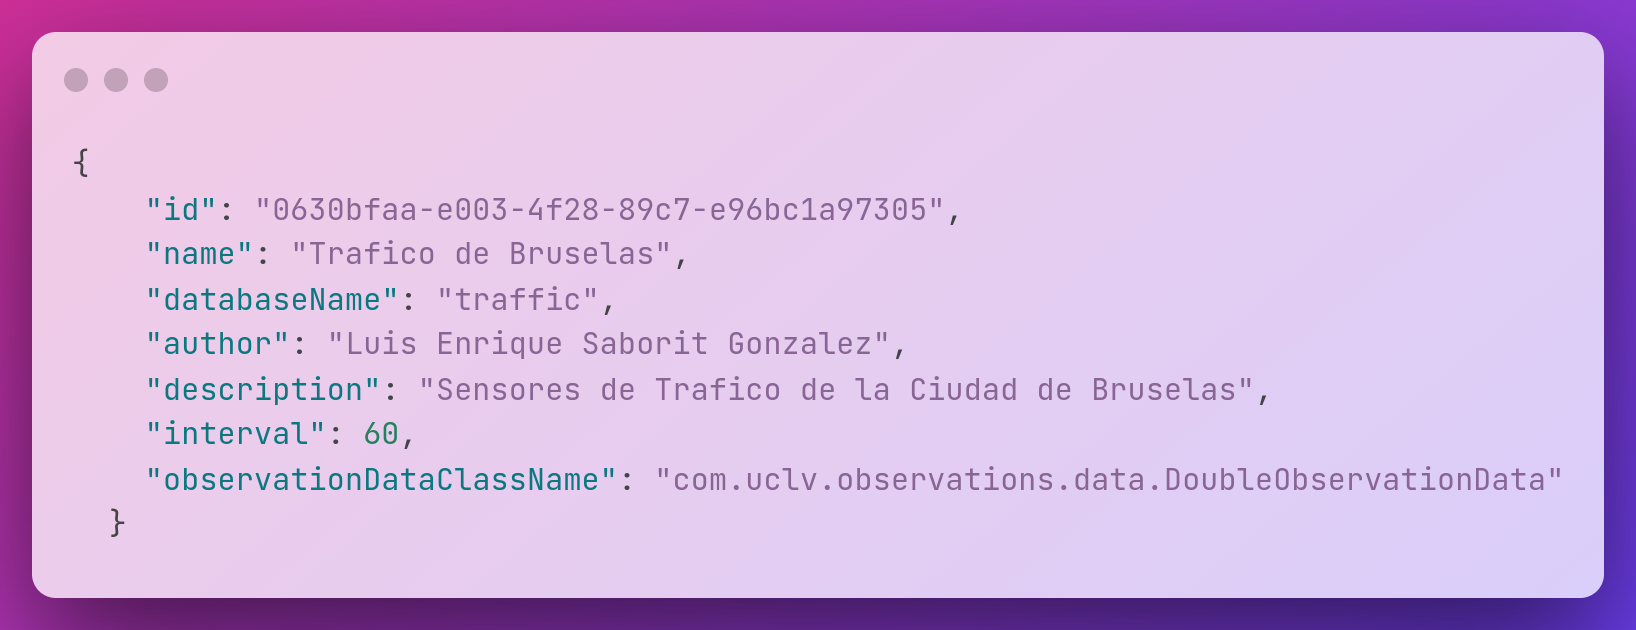
\includegraphics[width=0.8\textwidth]{imag/topic2.png}
    \caption{Un asunto en formato JSON}
    \label{fig:topic}
\end{figure}

La clase \textbf{Sensor} guarda un identificador del dispositivo, sus coordenadas geográficas, una descripción de lo que representan los datos que ofrece, la unidad de medida en la que se expresan estos datos y el asunto al que pertenece el sensor. La figura \ref{fig:uml_sensors} muestra las clases relacionadas con los sensores.

\begin{figure}[!ht]
    \centering
    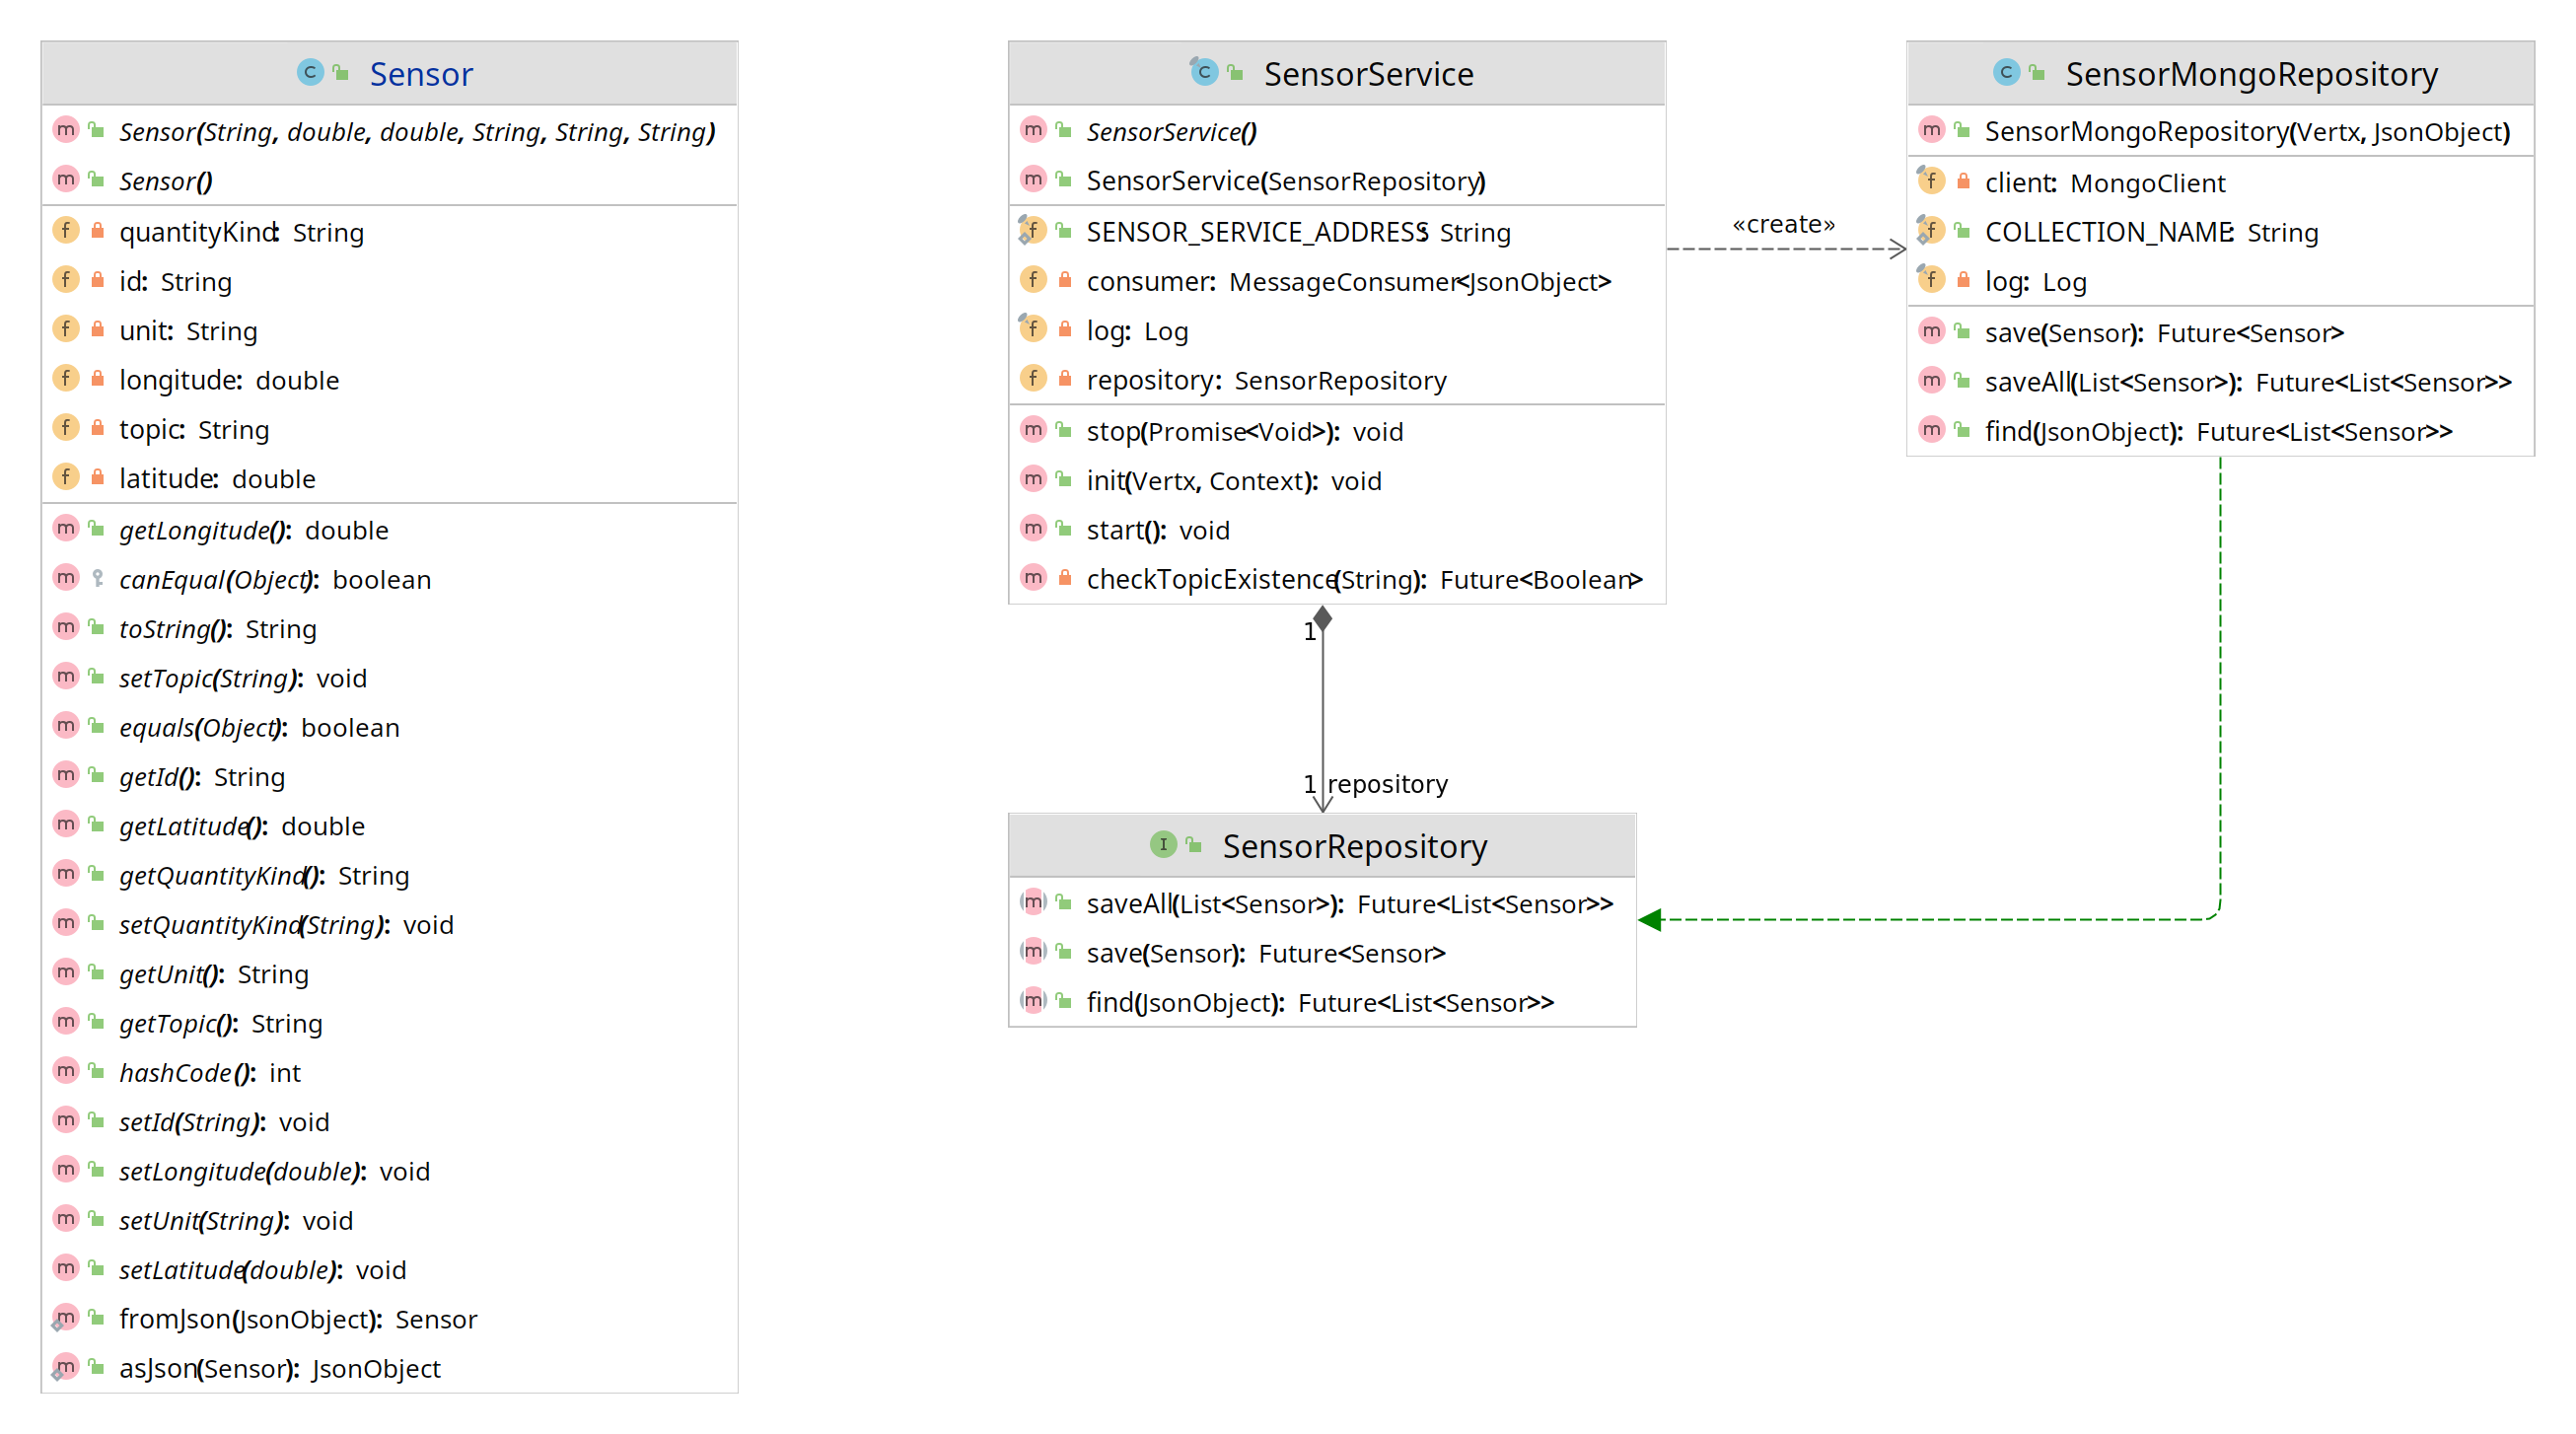
\includegraphics[width=\textwidth]{imag/uml_sensors.png}
    \caption{Clases relacionadas con los sensores}
    \label{fig:uml_sensors}
\end{figure}

La clase \textbf{SensorService} representa un servicio que gestiona los datos de los sensores. Para ello crea un repositorio en el que los guarda en formato JSON. La figura \ref{fig:sensor} muestra un ejemplo de tal representaci\'on. La clase \textbf{SensorMongoRepository} implementa el comportamiento de un repositorio que guarda datos de sensores. Este comportamiento est\'a definido en la interfaz \textbf{SensorRepository}.

\begin{figure}[!ht]
    \centering
    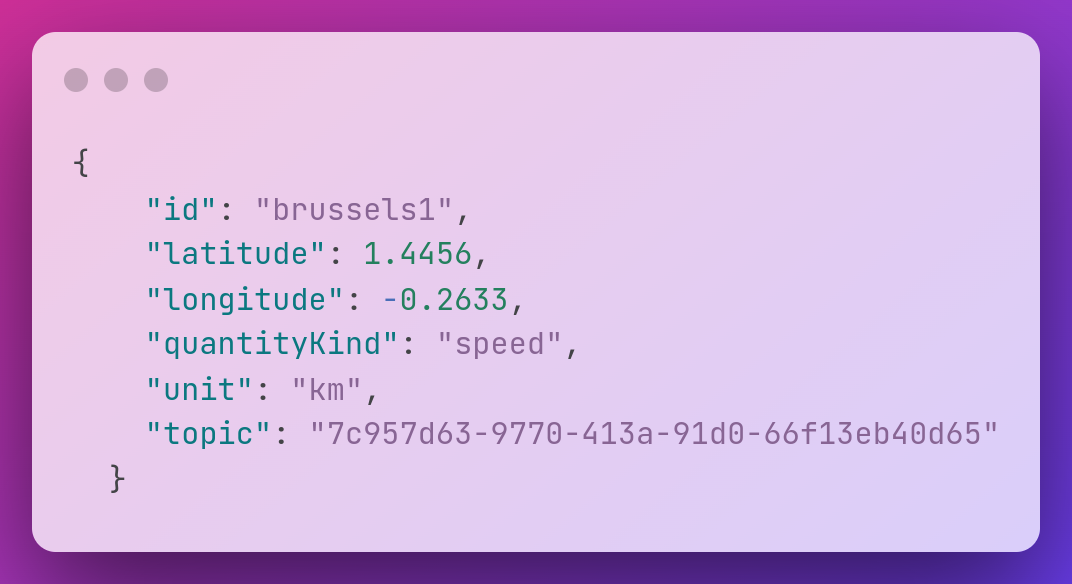
\includegraphics[width=0.5\textwidth]{imag/sensor2.png}
    \caption{Un sensor en formato JSON}
    \label{fig:sensor}
\end{figure}

De cada \textit{stream} (figura \ref{fig:uml_streams}) se guarda su identificador, el momento en que comenzó, el sensor que lo genera, la característica o \textit{feature} y su localización. Además la clase \textbf{Stream} posee un método que nos dice cuando dos \textit{stream}s son iguales. Al igual que con los sensores y los asuntos, existe una clase \textbf{StreamService} que representa un servicio que gestiona los datos de los \textit{streams}. La interfaz \textbf{StreamRepository} define el comportamiento de un repositorio de \textit{streams} mientras que la clase \textbf{StreamMongoRepository} lo implementa. 

\begin{figure}[!ht]
    \centering
    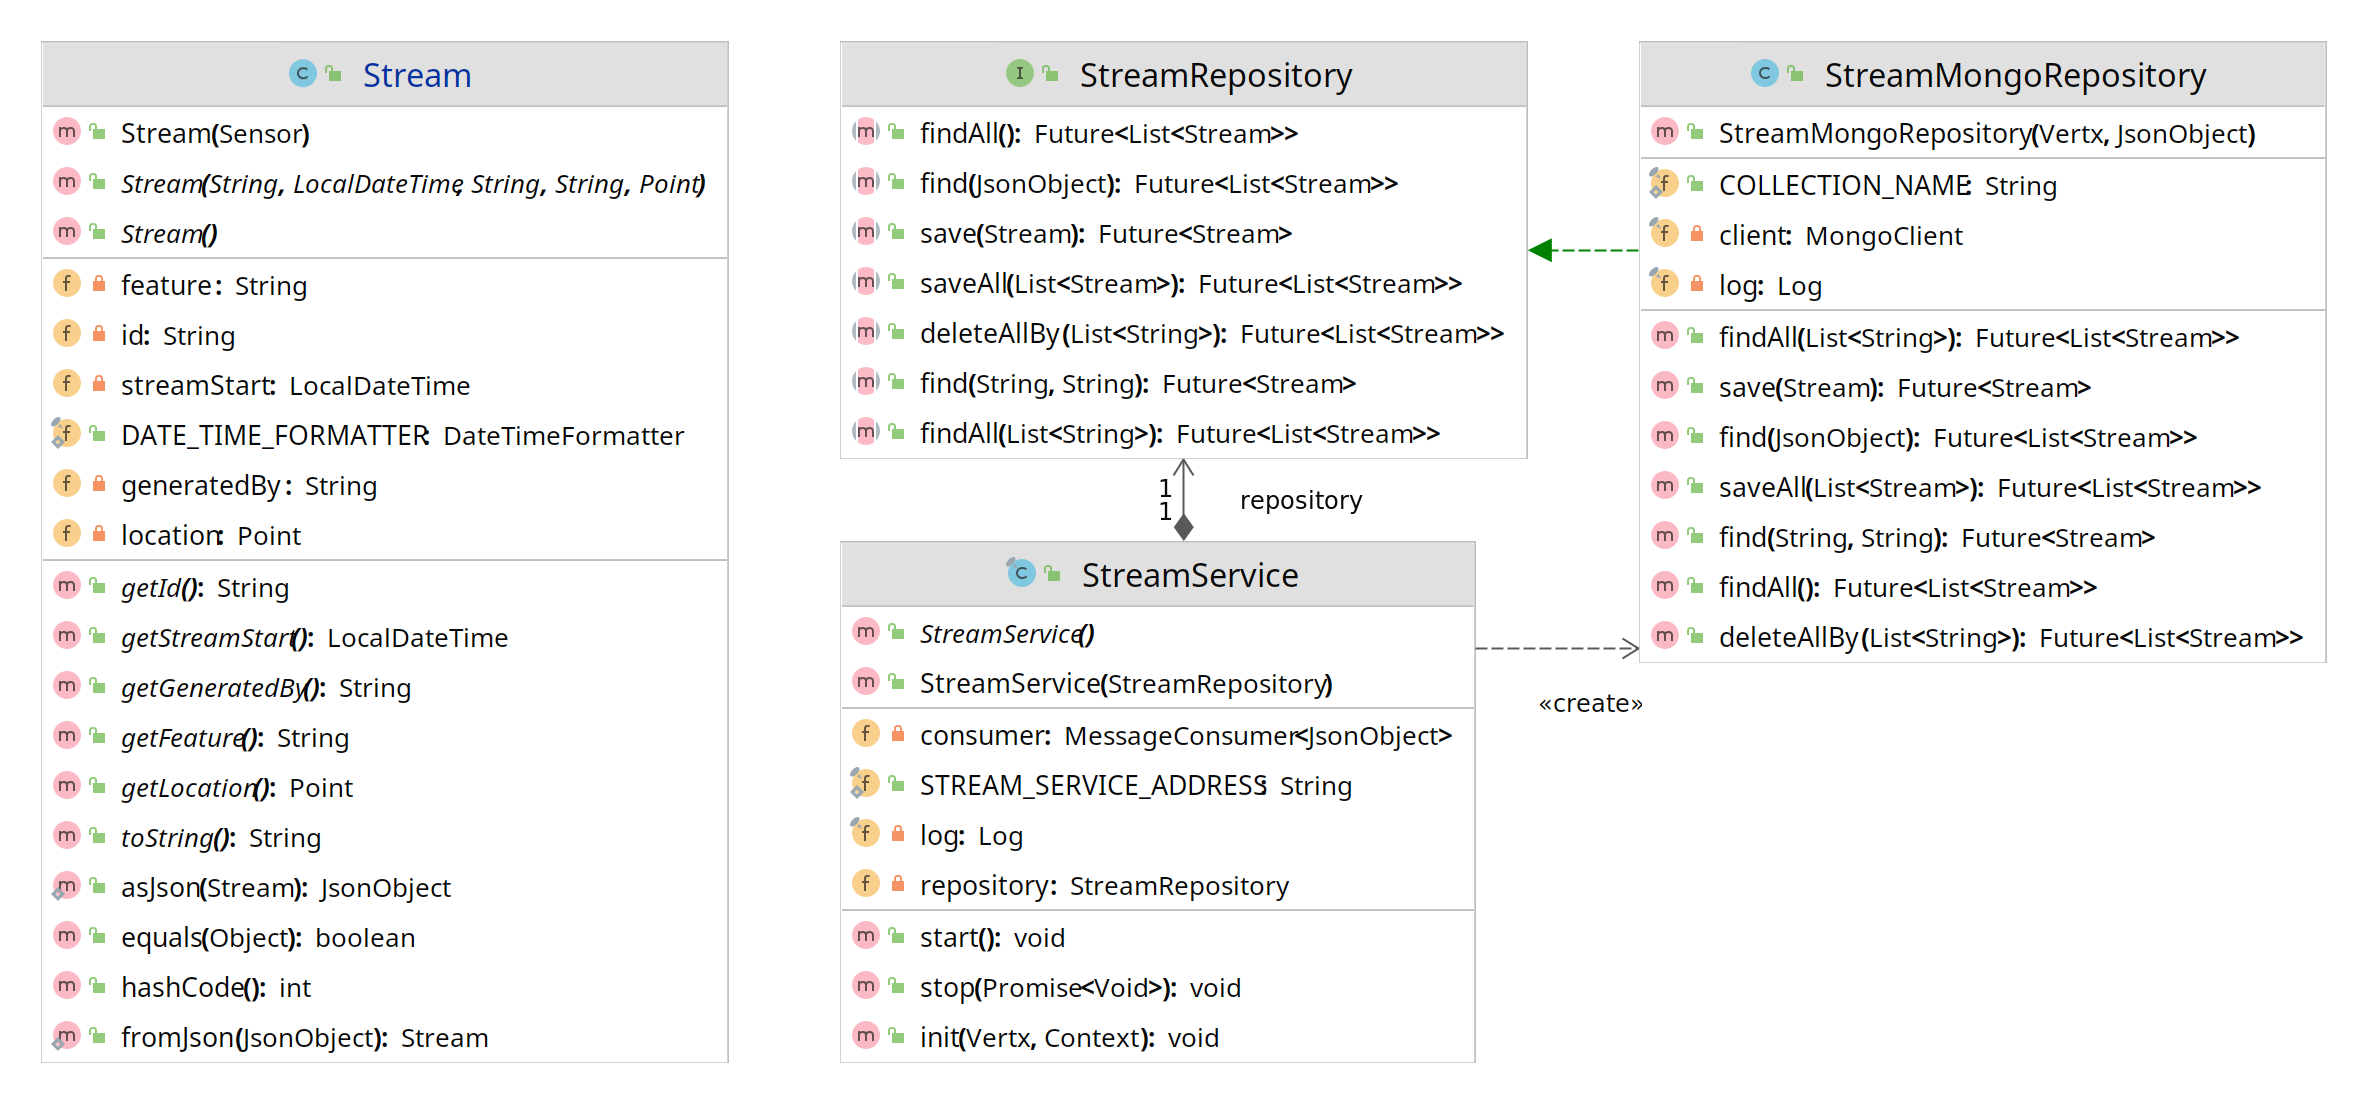
\includegraphics[width=\textwidth]{imag/uml_streams.png}
    \caption{Clases relacionadas con los streams}
    \label{fig:uml_streams}
\end{figure}

La figura \ref{fig:stream} muestra un \textit{stream} serializado a formato JSON con el objetivo de guardarlo en la base de datos.

\begin{figure}[!ht]
    \centering
    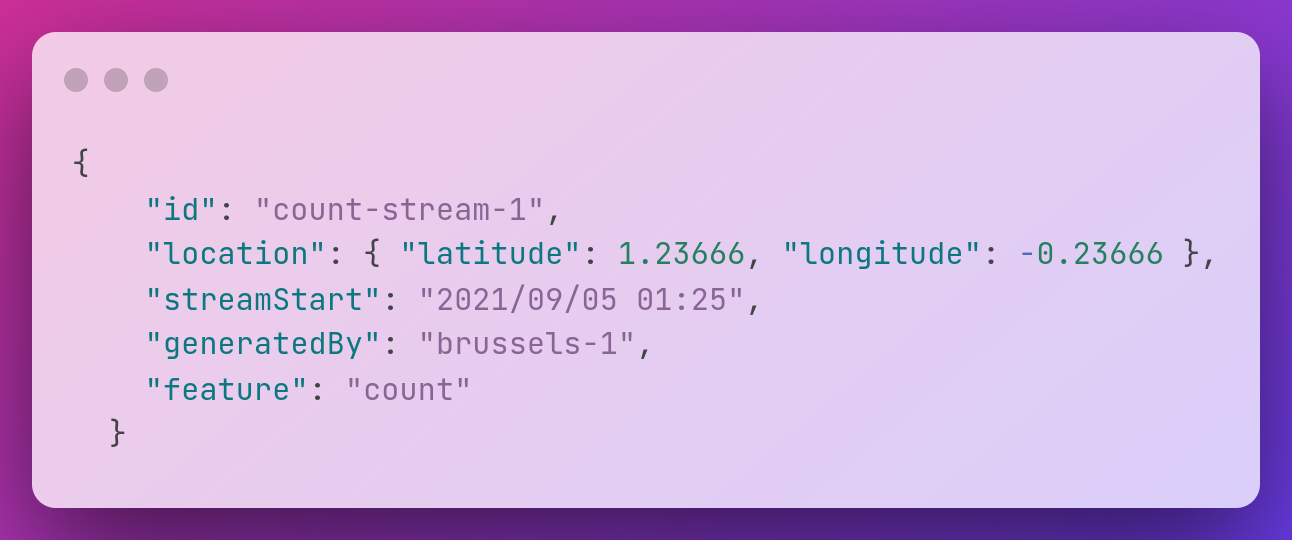
\includegraphics[width=0.6\textwidth]{imag/stream2.png}
    \caption{Un stream en formato JSON}
    \label{fig:stream}
\end{figure}

De cada observación se guarda un identificador, el \textit{stream} al que pertenece, el tiempo en el que se consiguió el resultado y el valor del dato de este resultado. Este valor puede ser de diferentes tipos.

Para lograr que el sistema pueda procesar los datos independientemente de la diversidad de tipos de datos de las mediciones, se introduce la interfaz \textbf{ObservationData}. Esta es una de las principales modificaciones que se le hicieron al sistema Traffic en este componente. Esta interfaz define el comportamiento de una clase que represente un valor de una observaci\'on y contiene, entre otros m\'etodos, los necesarios para convertir un objeto de la clase a formato JSON, o a crear una instancia de la clase a partir de un objeto en este formato.

\begin{figure}[!ht]
    \centering
    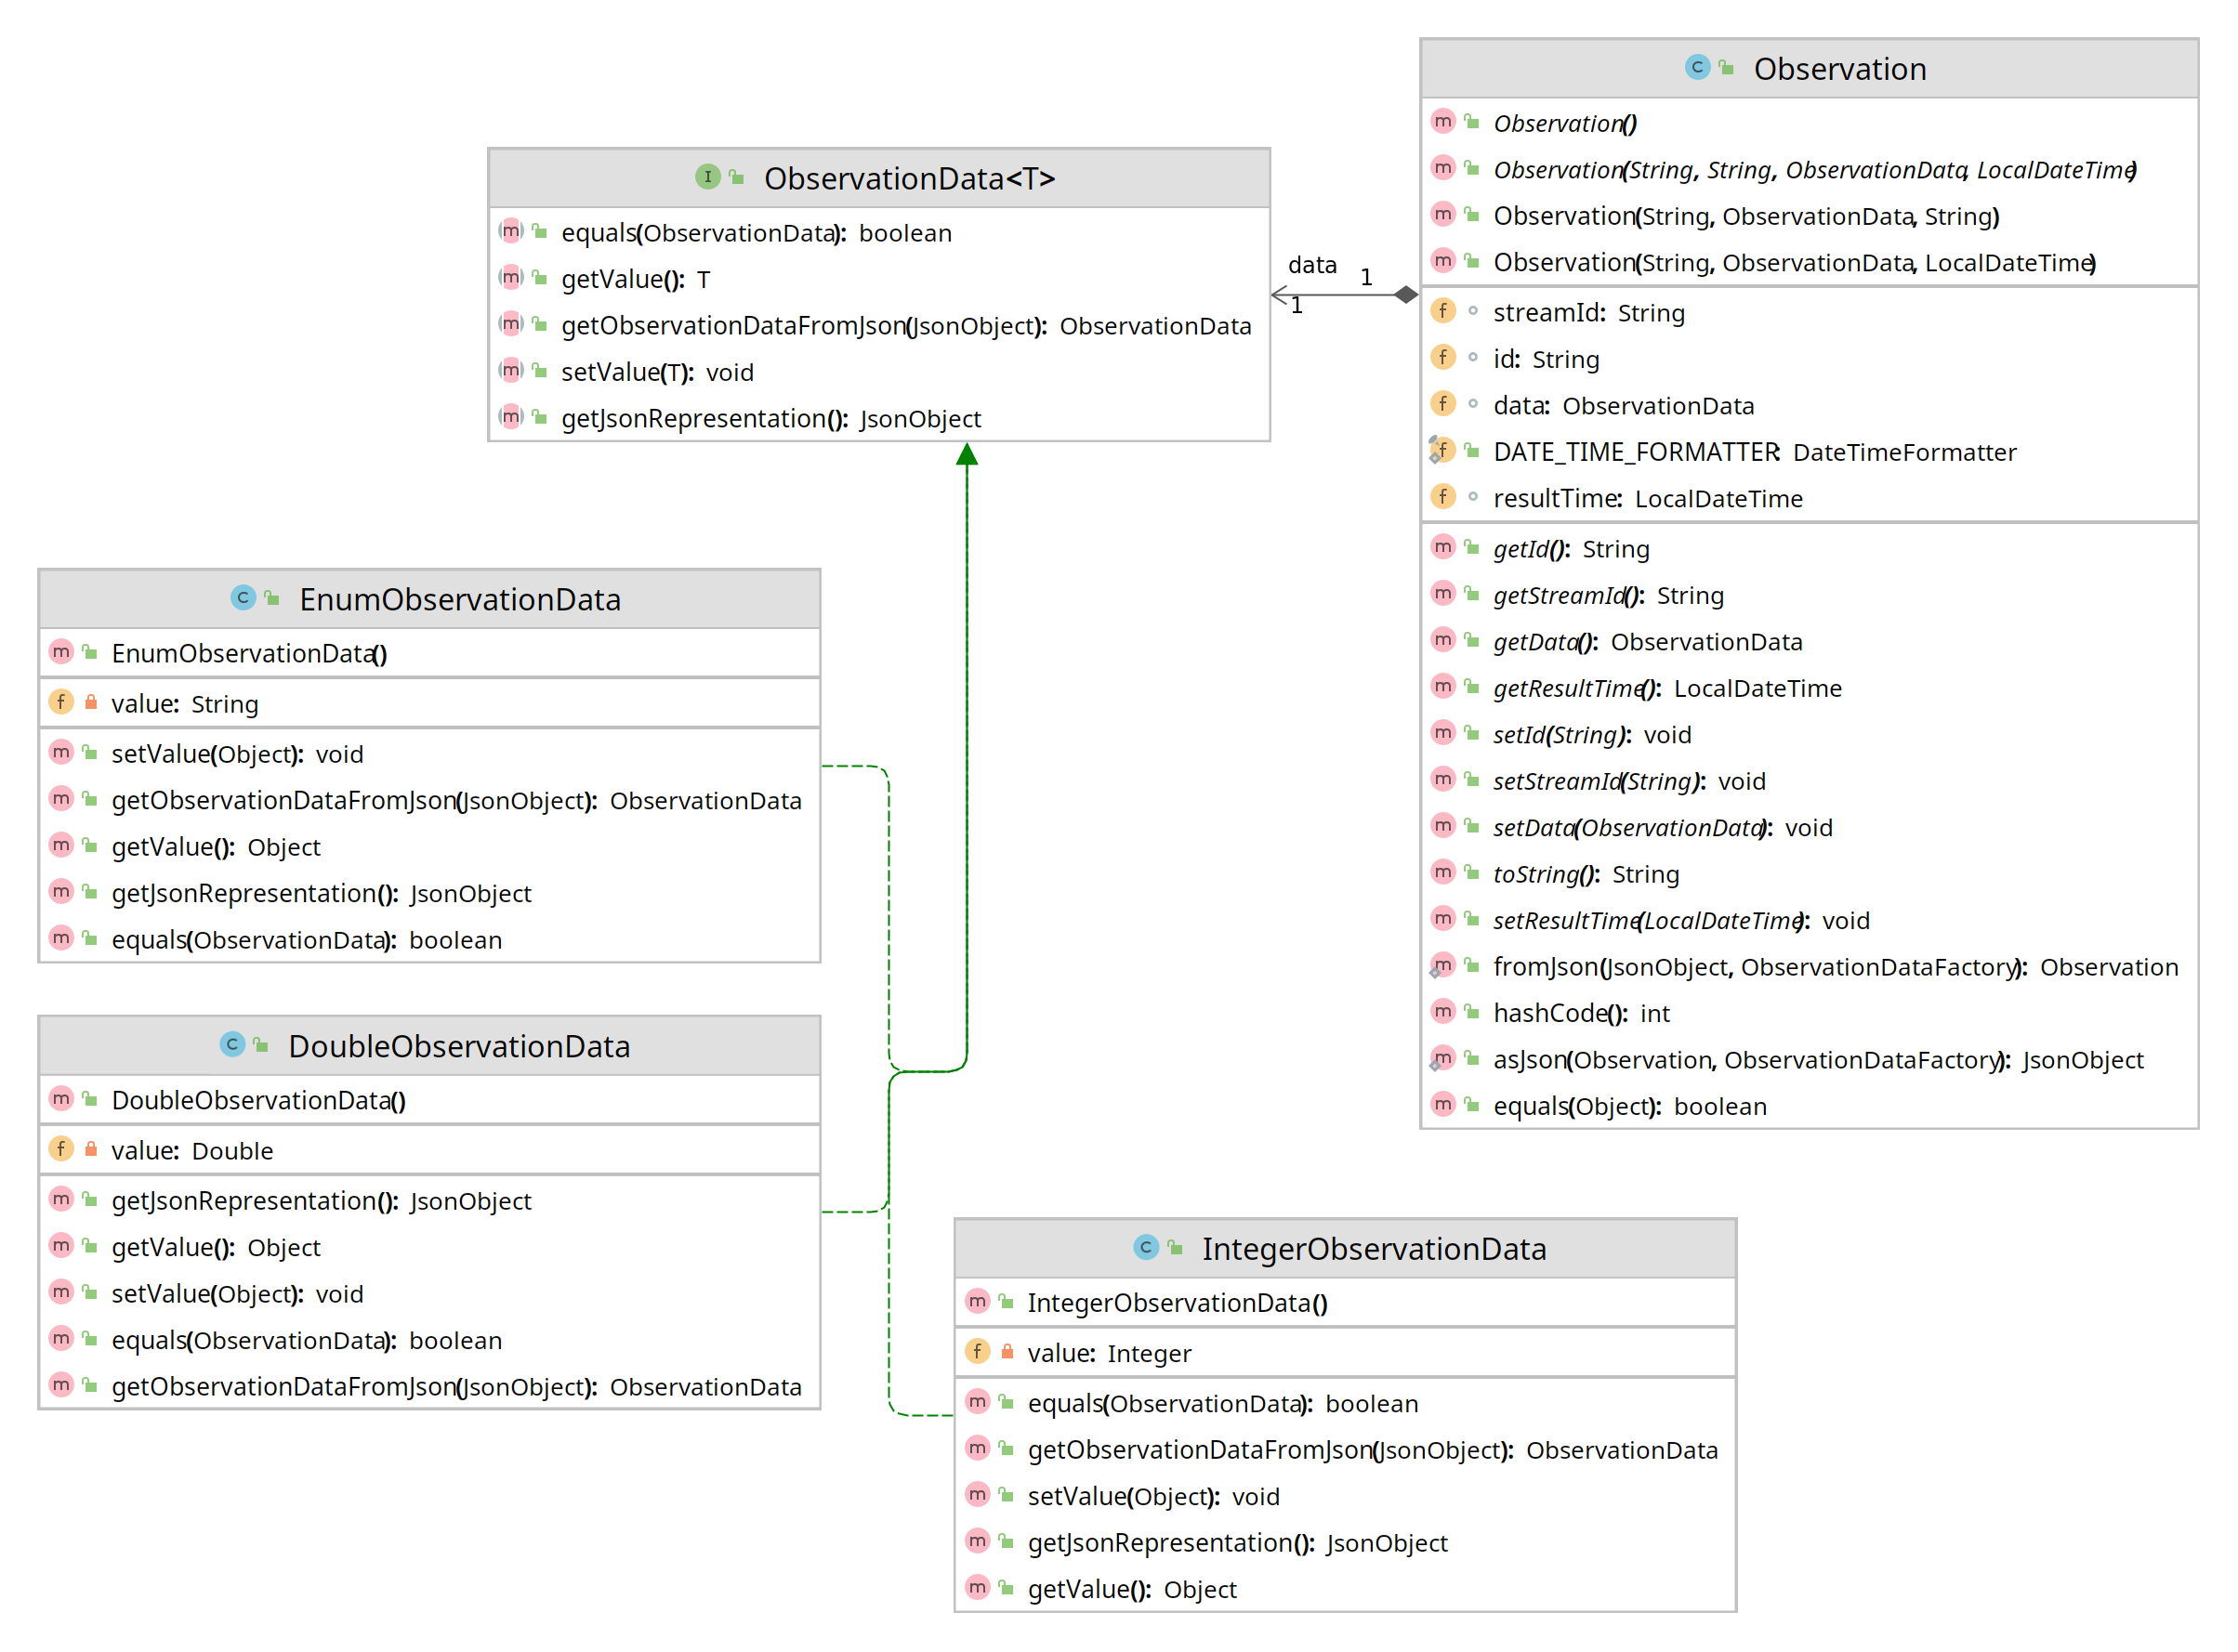
\includegraphics[width=\textwidth]{imag/uml_observationdata3.png}
    \caption{Diagrama de clases relacionadas con los diferentes tipos de observaciones}
    \label{fig:uml_observationdata}
\end{figure}

En el sistema, las clases \textbf{DoubleObservationData}, \textbf{IntegerObservationData} y \textbf{EnumObservationData} implementan la interfaz para los casos mencionados respectivamente, tal como se muestra en la figura \ref{fig:uml_observationdata}.


Las clases \textbf{ObservationService} y \textbf{ObservationLoggingService} representan servicios que gestionan las observaciones. El primero se encarga de publicarlas al br\'oker de mensajer\'ia, mientras el segundo las guarda en una base de datos \textbf{MongoDB} cuando sea necesario. El servicio \textbf{ObservationService} crea un repositorio \textbf{ObservationRedisRepository}, cuya clase implementa el comportamiento definido en \textbf{ObservationRepository} para un repositorio que gestiona observaciones. En este caso se trata de una conexi\'on a una base de datos \textbf{Redis}.

\begin{figure}[!ht]
    \centering
    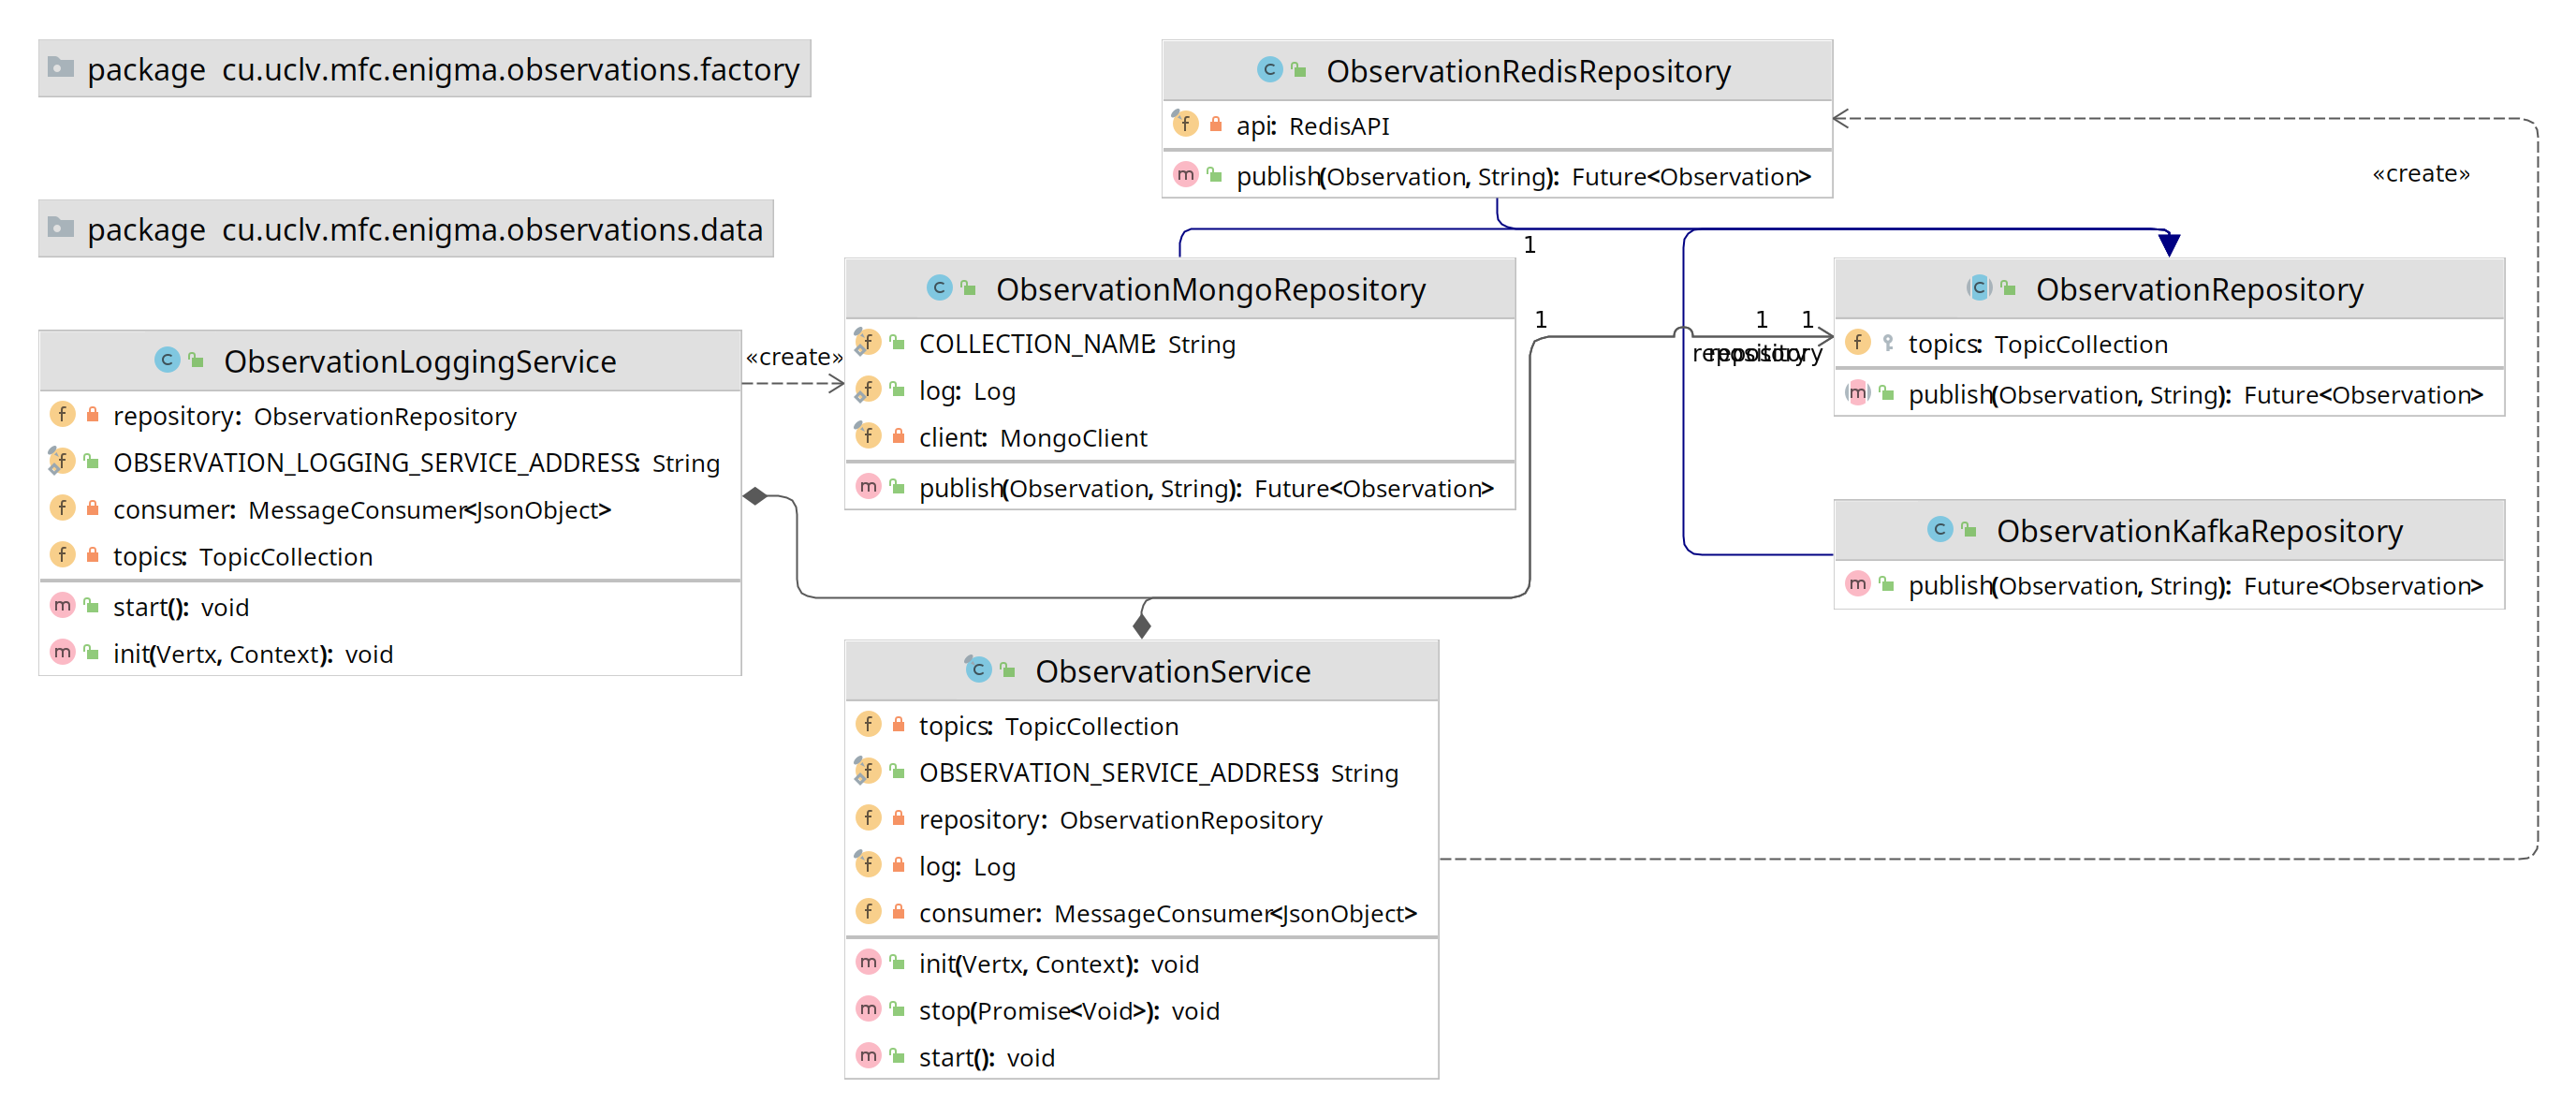
\includegraphics[width=\textwidth]{imag/uml_observations_package.png}
    \caption{Diagrama de las clases en el paquete de las observaciones}
    \label{fig:uml_observation_package}
\end{figure}

Se propone, como una modificaci\'on al sistema Traffic, agregar una clase \textbf{ObservationKafkaRepository}, que implemente el comportamiento usando una conexi\'on a una instancia de \textbf{Apache Kafka}, una plataforma distribuida de transmisión de eventos. El componente Br\'oker de Mensajer\'ia debe pasar de usar la base de datos \textbf{Redis} a usar \textbf{Kafka} para permitir que los dem\'as componentes puedan publicar datos y suscribirse a \textit{streams} de forma m\'as fiable, y que la informaci\'on pueda persistirse por m\'as tiempo. El diagrama de clases correspondiente, se muestra en la figura \ref{fig:uml_observation_package}.

El \textbf{ObservationLoggingService} por su parte, usa un objeto de la clase \textbf{ObservationMongoRepository} para publicar las observaciones a un repositorio \textbf{MongoDB}. Esta clase hereda el comportamiento de la clase abstracta \textbf{ObservationRepository}.

En la figura \ref{fig:observation} se muestra como quedar\'ia una observaci\'on que usa datos del tipo \textbf{DoubleObservationData}, convertida a formato JSON.

\begin{figure}[!ht]
    \centering
    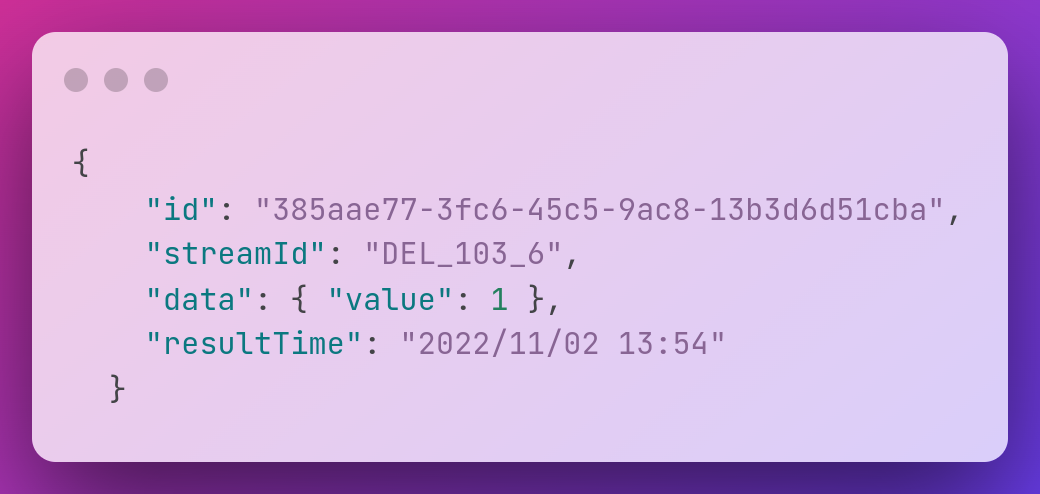
\includegraphics[width=0.6\textwidth]{imag/observation2.png}
    \caption{Una observaci\'on en formato JSON}
    \label{fig:observation}
\end{figure}


\end{comment}

\newpage
\vspace*{3cm}

\begin{comment}

\section[Utilizaci\'on de la plataforma en un caso de uso espec\'ifico]{\texorpdfstring{Cap\'itulo 3:\\ Utilizaci\'on de la plataforma en un\\ caso de uso espec\'ifico}{Cap\'itulo 3:\\ Utilizaci\'on de la plataforma en un\\ caso de uso espec\'ifico}}
\vspace*{1cm}


En este cap\'itulo se enumeran los pasos para adaptar la plataforma a un caso de uso espec\'ifico. Adem\'as, se describe la API del Componente Principal. Por \'ultimo, se explican el proceso de despliegue del sistema y las pruebas realizadas para evaluar su desdempe\~no.

\subsection{Primeros pasos para el uso de la plataforma}

Para adaptar la plataforma  a un caso de uso espec\'ifico, comenzamos por crear un asunto en el cual se define el tipo de datos de los resultados de las observaciones. Esto se logra mediante una petici\'on a la API de la plataforma, o mediante una p\'agina web desarrollada como elemento consumidor.  

Se sugiere programar un \textit{script} o programa auxiliar que obtenga los datos de la fuente, los procese, los convierta al formato JSON requerido por la plataforma y luego los publique a la API. En el repositorio de \textbf{github} del proyecto \footnote{\href{https://github.com/Saborit10/thesis}{https://github.com/Saborit10/thesis}}, se encuentra el \textit{script}, escrito en Python, utilizado para obtener datos de los sensores de tr\'afico de la ciudad de Bruselas, usados por el sistema Traffic.

Este \textit{script} debe primero procesar los datos de los sensores y \textit{streams}, y luego hacer peticiones peri\'odicas a la fuente para obtener las observaciones. 

Una vez que los datos son publicados peri\'odicamente a la plataforma, en dependencia de las necesidades del caso espec\'ifico, se puede programar un servicio de analíticas externo que se comunique con la plataforma a través de la API y que pueda entre otras cosas, publicar a esta los eventos que ocurran en los flujos de datos.

\subsection{Descripción de la API}

Para establecer una forma \'unica en la que los datos son introducidos a la plataforma, se ha implementado una API a la que se puede publicar información y a través de la cual se pueden obtener datos acerca de los flujos. Toda la información está en formato JSON.

Las respuestas a las solicitudes contienen la propiedad \texttt{status}. Si la solicitud fue procesada con \'exito, \texttt{status} es igual a \texttt{OK} y el objeto contiene una propiedad llamada \texttt{data}, la cual contiene la respuesta. En caso contrario, \texttt{status} ser\'a igual a \texttt{FAIL} y el objeto contendr\'a una propiedad llamada \texttt{cause}, que es un mensaje con la causa del fallo en la petici\'on.

A continuaci\'on se describen algunos de los m\'etodos POST:

\begin{itemize}
    \item {
        \texttt{/api/addtopic} Agrega un asunto al sistema. El asunto debe seguir un formato como el que se aprecia en la figura \ref{fig:example_addtopic}. Si la solicitud es exitosa, el m\'etodo devuelve como respuesta el objeto recibido.
        
        \begin{figure}[H]
            \centering
            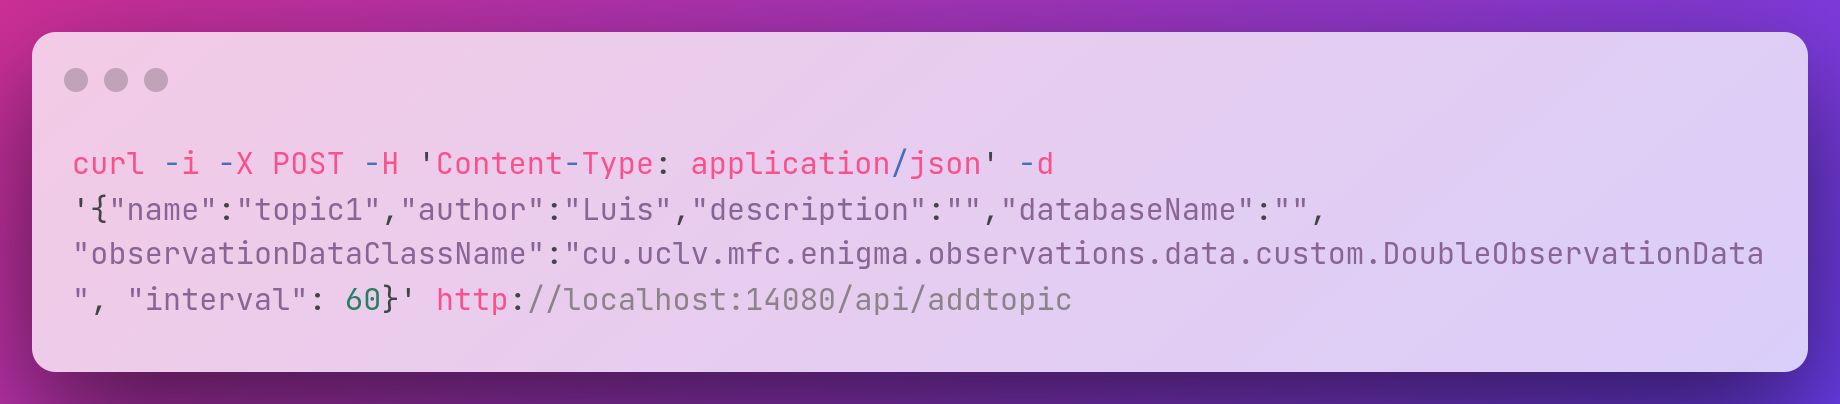
\includegraphics[width=\textwidth]{imag/example_addtopic2.png}
            \caption{Ejemplo de solicitud para agragar un asunto}
            \label{fig:example_addtopic}
        \end{figure}
    }
    \item {
        \texttt{/api/addsensor} Agrega un sensor al sistema. El sensor debe seguir un formato como el que se aprecia en la figura \ref{fig:example_addsensor}. Si el identificador del asunto especificado en el sensor no pertenece a un asunto en el sistema, la solicitud falla. Si la solicitud es exitosa, el m\'etodo devuelve como respuesta el objeto recibido.

        \begin{figure}[!ht]
            \centering
            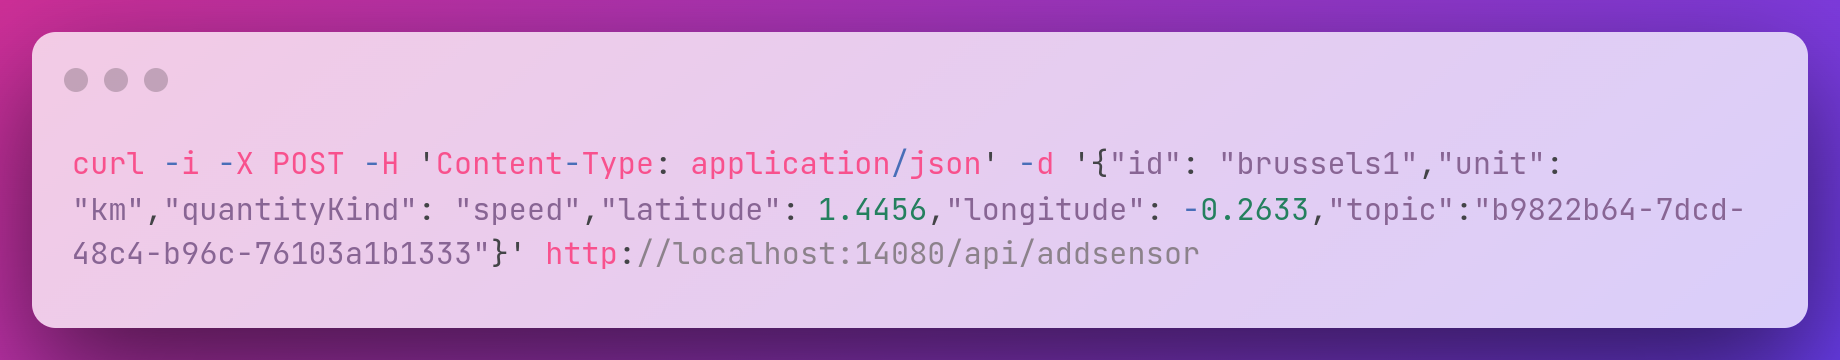
\includegraphics[width=\textwidth]{imag/example_addsensor2.png}
            \caption{Ejemplo de solicitud para agragar un sensor}
            \label{fig:example_addsensor}
        \end{figure}
    }
    \item {
        \texttt{/api/addstream} Agrega un \textit{stream} al sistema. El stream debe seguir un formato como el que se aprecia en la figura \ref{fig:example_addstream}. Si la solicitud es exitosa, el m\'etodo devuelve como respuesta el objeto recibido.

        \begin{figure}[!ht]
            \centering
            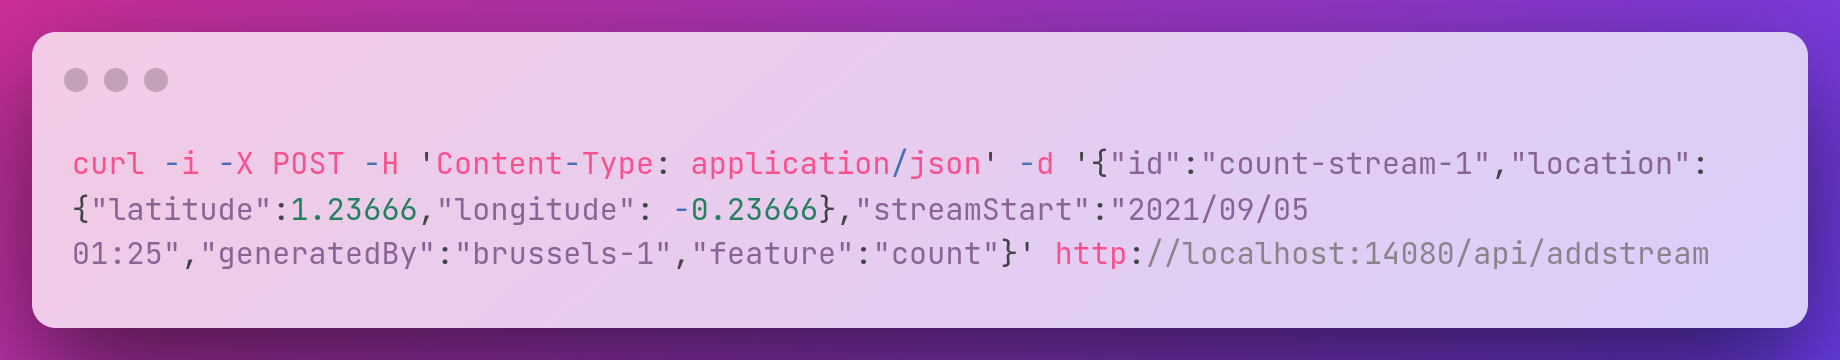
\includegraphics[width=\textwidth]{imag/example_addstream2.png}
            \caption{Ejemplo de solicitud para agragar un \textit{stream}}
            \label{fig:example_addstream}
        \end{figure}
    }
    \item {
        \texttt{/api/addobservation} Agrega una observaci\'on al sistema. La observaci\'on debe seguir un formato como el que se aprecia en la figura \ref{fig:example_addobservation}. Si la solicitud es exitosa, el m\'etodo devuelve como respuesta el objeto recibido.

        \begin{figure}[H]
            \centering
            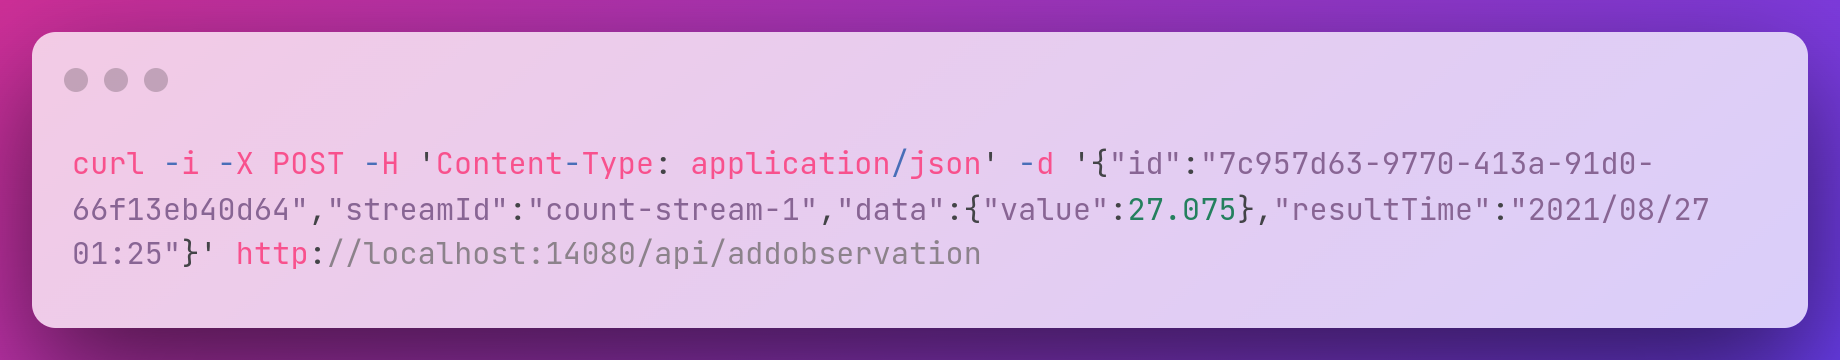
\includegraphics[width=\textwidth]{imag/example_addobservation2.png}
            \caption{Ejemplo de solicitud para agragar una observaci\'on}
            \label{fig:example_addobservation}
        \end{figure}
    }
\end{itemize}

\vspace{1cm}

A continuaci\'on se describen algunos de los m\'etodos GET:
\begin{itemize}
    \item {
        \texttt{/api/topicSensors/\{topicId\}} Devuelve todos los sensores que pertenecen a un asunto cuyo identificador es \texttt{topicId}. Un ejemplo de la solucitud se muestra en la figura \ref{fig:example_topicSensors}.
        
        \begin{figure}[!ht]
            \centering
            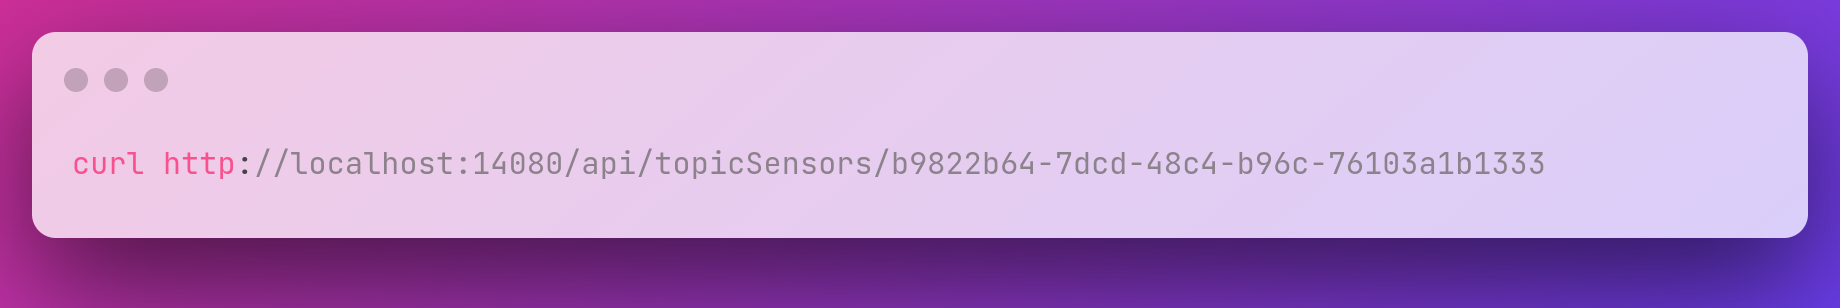
\includegraphics[width=\textwidth]{imag/example_topicSensors2.png}
            \caption{Ejemplo de solicitud para obtener todos los sensores correspondientes a un asunto}
            \label{fig:example_topicSensors}
        \end{figure}
    }
\end{itemize}

A medida que se implementen los dem\'as componentes de la plataforma, deben agregarse m\'as \textit{endpoints} a la API. Por ejemplo, para pedir desplegar servicios de anal\'iticas y para iniciar la comunicaci\'on con el br\'oker de mensajer\'ia. 


\subsection{Despliegue de la Plataforma}

Aunque en la etapa de desarrollo y en las pruebas realizadas al sistema se desplegaron todos los componentes usados en la misma computadora o nodo, al desplegar el sistema para su funcionamiento se recomienda distribuir estos elementos en diferentes dispositivos, contribuyendo as\'i a su escalabilidad.

La figura \ref{fig:diagrama_despliegue} muestra una posible distribuci\'on de los componentes. Se tiene el Componente Pricipal, un servidor \textbf{MongoDB} y el br\'oker de mensajer\'ia (\textbf{Apache Kafka}) en sus respectivos nodos. Los dos \'ultimos servicios deben ser desplegados preferiblemente usando \textbf{Docker}.

El componente de registro y la base de datos \textbf{Stardog} se despliegan en un mismo nodo.

\begin{figure}[!ht]
    \centering
    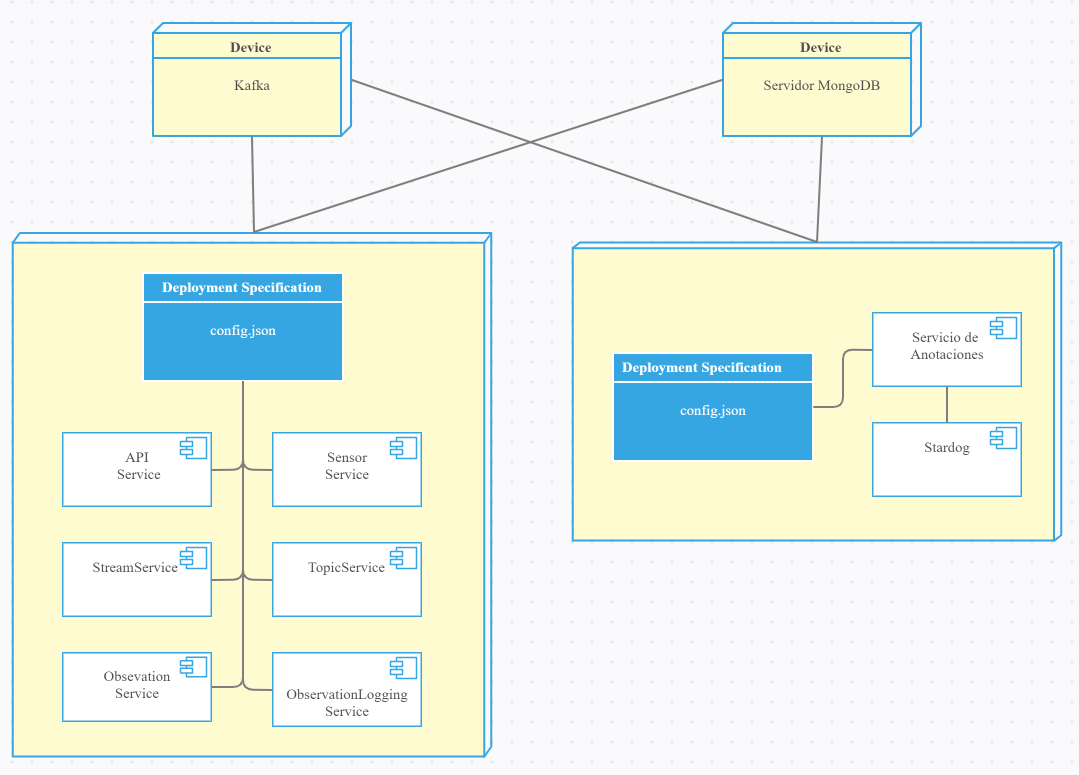
\includegraphics[width=\textwidth]{imag/diagrama_despliegue.png}
    \caption{Diagrama de despliegue de la plataforma}
    \label{fig:diagrama_despliegue}
\end{figure}


\subsection{Pruebas Realizadas al Sistema}
Al sistema se le realizaron varias pruebas para evaluar su desempe\~no. Por ejemplo, se realizaron pruebas unitarias a diferentes funcionalidades. Este tipo de pruebas se enfoca en caracter\'isticas y operaciones espec\'ificas. Son altamente automatizables e independientes.

En el proceso, se utiliz\'o \textbf{JUnit5}, un \textit{framework} para pruebas unitarias en Java. Adem\'as se utilizaron herramientas de \textbf{Vert.x} para realizar las pruebas al c\'odigo que se comporta de forma as\'incrona.

Se pueden llevar a cabo varias pruebas unitarias. Por ejemplo, se puede comprobar que un sensor o un \textit{stream} se agrege al repositorio de forma satisfactoria, que los m\'etodos \texttt{fromJson} y \texttt{asJson} conviertan los datos de un formato a otro sin problemas, o que las operaciones de buscar datos en los repositorios funcionen de forma correcta.

A continuaci\'on (figura \ref{fig:unit_tests}) se muestran los resultados para los dos primeros ejemplos.

\begin{figure}[!ht]
    \centering
    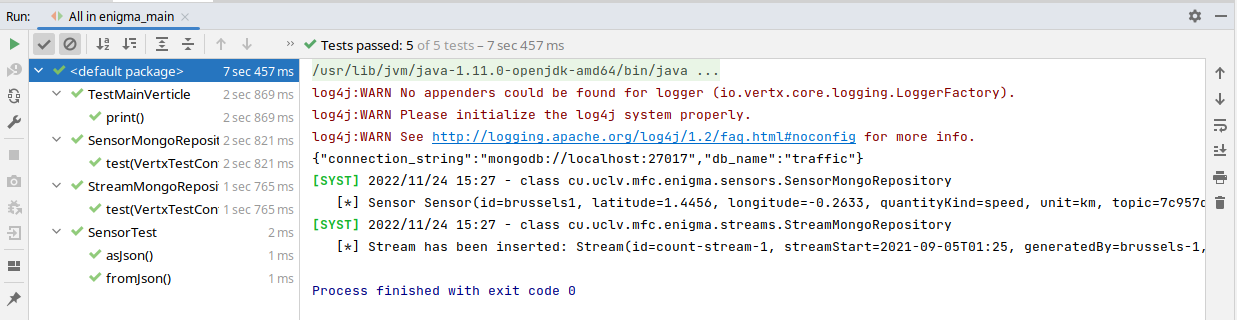
\includegraphics[width=\textwidth]{imag/unit_tests.png}
    \caption{Resultados de las pruebas unitarias}
    \label{fig:unit_tests}
\end{figure}

Como se puede apreciar en la figura, el sistema pasa todas las pruebas realizadas. En el panel de la derecha podemos observar la salida de la plataforma.

Tambi\'en se realizaron pruebas de rendimiento al sistema. En la primera prueba se simula el trabajo de la plataforma en un \'unico caso de uso. Para ello se usa un \textit{script} escrito en Python que crea un asunto, hace peticiones a la fuente de datos, procesa la informaci\'on y publica esta a la API de la plataforma. Se hace una primera petici\'on para obtener los datos de los sensores y luego se realiza otra cada sesenta segundos. Cada tarea de este tipo se realiza en su propio hilo de ejecuci\'on.

En la segunda prueba se crearon veinte instancias en la plataforma. Para cada instancia se hizo un trabajo similar al de la primera prueba, pero en esta oportunidad, las peticiones de todos los casos de uso se hicieron a la vez, y se publicaron a la plataforma al mismo tiempo. Esto se hace con el objetivo de medir la estabilidad del sistema en los picos de procesamiento.

En la figura \ref{fig:prueba_rendimiento} se observa el consumo de recursos mediante las pruebas de rendimiento, para la plataforma desplegada en una computadora \textit{Intel Core i3-4160 @ 4x 3.6GHz} de \textit{8Gb} de memoria RAM, con sistema operativo \textit{Debian 11}.

\begin{figure}[!ht]
    \centering
    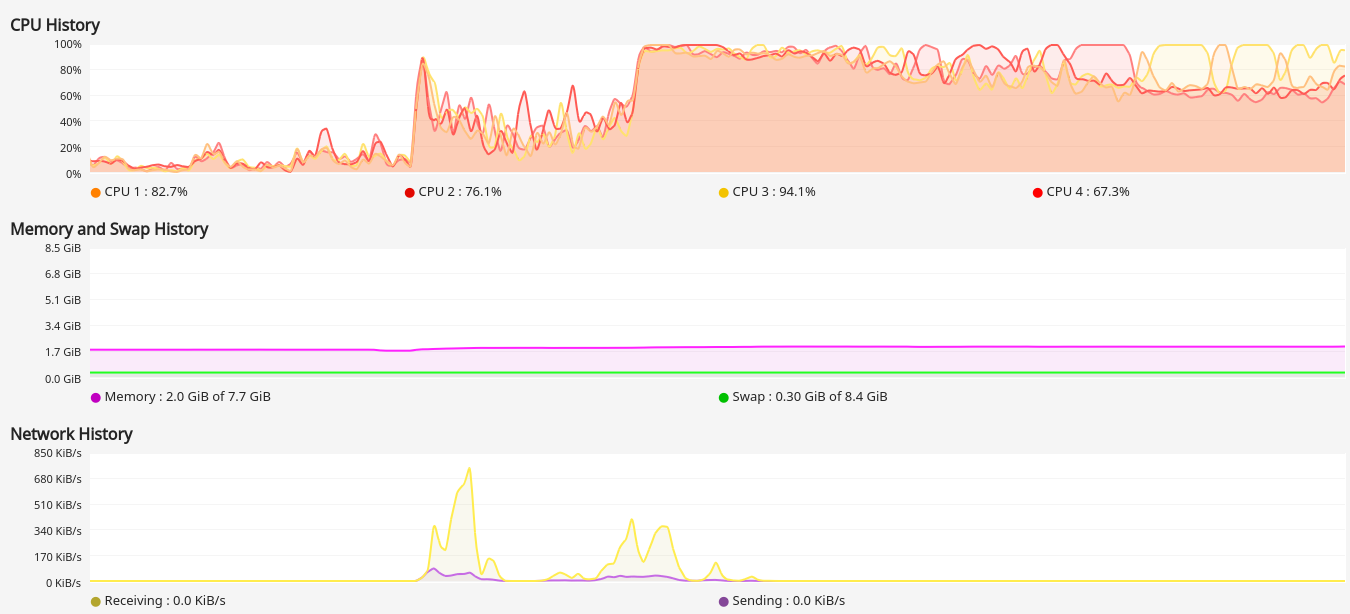
\includegraphics[width=\textwidth]{imag/rendimiento_prueba2.png}
    \caption{Recursos del sistema durante una prueba de rendimiento}
    \label{fig:prueba_rendimiento}
\end{figure}

Se aprecia que el sistema no agota todos los recursos de \textit{hardware}, incluso cuando se hacen todas las peticiones al un\'isono.

Los tiempos de respuesta del sistema en las pruebas realizadas son:

\begin{itemize}
    \item {
        El máximo tiempo de respuesta de una petición a la API, la cual crea un asunto es 0.031 segundos.
    }
    \item {
        El máximo tiempo de respuesta de una petición a la API, la cual publica un sensor es 0.821 segundos.
    }
    \item {
        El máximo tiempo de respuesta de una petición a la API, la cual publica un stream es 0.915 segundos.
    }
\end{itemize}

Al analizar los dos \'ultimos resultados, aunque a primera vista pueden parecer elevados, debemos tener en cuenta que se trata de los tiempos m\'aximos de ejecuci\'on de m\'as de $4000$ peticiones que compiten por ser procesadas por la API al un\'isono. Al desplegar la plataforma para su uso, estas operaciones se realizar\'an distribuidas en varios instantes de tiempo. 

Todos los \textit{scripts} y los c\'odigos de las pruebas realizadas pueden encontrarse en el repositorio de GitHub antes mencionado.




\newpage
\vspace*{3cm}
\section*{Conclusiones}
\vspace*{1cm}

\noindent Como resultado de este trabajo se arriban a las conclusiones siguientes:
\begin{itemize}
    \item {
        Se establecen como requisitos principales de la plataforma ENIGMA la adaptabilidad y extensibilidad, esta plataforma está integrada por cinco componentes construidos en forma de servicios por lo que esta arquitectura permite un despliegue distribuido de sus componentes.
    }
    \item {
        Se han implementado las clases y los servicios que integran la componente Principal de la plataforma ENIGMA y a manera de evaluación del diseño y la implementación se ha instanciado este componente para procesar un flujo concreto.
    }
    \item {
        Se definió y aplicó una estrategia de evaluación para la componente implementada, los resultados de esta evaluación basadas en pruebas fueron satisfactorias.
    }
\end{itemize}

Por lo anterior se puede afirmar que se ha logrado cumplir el objetivo general propuesto en este trabajo de desarrollar la Componente Principal de la plataforma ENIGMA.



% Despu\'es de realizar las pruebas descritas, se puede concluir que el sistema funciona correctamente al procesar varias instancias (en este caso veinte). Al usar un paradigma de programaci\'on as\'incrono, las operaciones no bloquean el flujo de trabajo. De esta forma se logra que varias de ellas puedan realizarse al mismo tiempo.




\newpage
\vspace*{3cm}
\section*{Recomendaciones}
\vspace*{1cm}


\noindent Para dar continuidad a este trabajo se recomienda:
\begin{itemize}
    \item {
        Realizar pruebas del Componte Principal en entornos más reales y diversos.
    }
    \item {
        Trabajar para lograr que el Componente Principal pueda procesar información de cualquier tipo de dato definido por el usuario que adapta la plataforma a su caso espec\'ifico.
    }
    \item {
        Continuar con la implementación de los restantes componentes de la plataforma.
    }
\end{itemize}

\end{comment}

\newpage
\vspace*{3cm}
% \section*{Bibliograf\'ia}

%\bibliographystyle{ieeetr}
%\bibliographystyle{agsm} 
\bibliographystyle{abbrvnat}
% \setcitestyle{authoryear,open={((},close={))}} 

\bibliography{ref}

% \vspace*{1cm}



\end{document}
